\setbeamertemplate{headline text style}{\Tiny}%

\begin{bibunit}[apalike]

\part[author={Stéphane GALLAND},label={chap:intermediate_code_generation}]{Intermediate Code Generation}

\tableofcontentslide

\section{Introduction}

\begin{frame}{Introduction}
	\vfill
	\begin{itemize}
	\item This chapter develops two major points:
		\vfill
		\begin{enumerate}
		\item The translation of languages guided by context-free grammars.
		\vfill
		\item These translation techniques are applied to type checking and intermediate code generation.
		\end{enumerate}
	\end{itemize}
	\vfill
	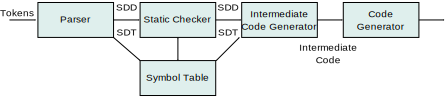
\includegraphics[width=\linewidth]{parser_toolchain}
\end{frame}

\sidecite{Samelson.1960, Brooker.1962}
\begin{frame}{Syntax-Directed Translation}
	\begin{itemize}
	\item A \emph{syntax-directed translation} specifies the values of attributes, attached to the grammar symbols, by associating semantic rules with the grammar productions.
		\begin{sdd}
		\p{expr ::= expr \tok+ term}{head.t = expr.t \concat term.t \concat '+'}
		\p{     ::= expr \tok- term}{head.t = expr.t \concat term.t \concat '-'}
		\p{     ::= term}{head.t = term.t}
		\p{term ::= \tok0}{head.t = '0'}
		\p{     ::= \tok1}{head.t = '1'}
		\pdots
		\p{     ::= \tok9}{head.t = '9'}
		\end{sdd}
	\vspace{1em}
	\item A Syntax-directed translation scheme embeds program fragments (or semantic actions, between braces) inside the semantic rules.
	\end{itemize}
\end{frame}

\begin{frame}{Two Types of Syntax-Directed Translation}
	\begin{itemize}
	\item The most general approach to syntax-directed translation is:
		\begin{itemize}
		\item to construct a parse tree, and
		\item then to compute the values of the attributes at the nodes of the tree by visiting the nodes.
		\end{itemize}
	\vfill
	\item In many cases, translation can be done during parsing, without building an explicit tree.
	\vfill
	\item Two classes of syntax-directed translation are presented:
		\begin{itemize}
		\item \emph{L-attributed translations} (L=left)
		\item \emph{S-attributed translations} (S=synthesized)
		\end{itemize}
	\end{itemize}
\end{frame}

\begin{frame}{Program Checking}
	\begin{itemize}
	\item Static checking includes \emph{type checking}, which ensures that operators are applied to compatible operands.
	\vspace{4em}
	\item It also includes any \emph{syntactic checks} that remain after parsing.
	\end{itemize}
\end{frame}

\begin{frame}{Intermediate Representation}
	\begin{itemize}
	\item In the process of translating a program in a given source language into code for a given target machine, a compiler may construct a sequence of intermediate representations. \\
	\vfill
		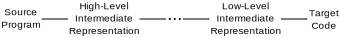
\includegraphics[width=\linewidth]{intermediate_representations}
	\vfill
	\item High-level representation is close to the source language \eg syntax tree.
	\item Low-level representation are close to the target machine \eg three-address code.
	\end{itemize}
\end{frame}

\section{Translation scheme}

\tableofcontentslide[sections={1-4},sectionstyle={show/shaded},subsectionstyle={show/show/hide},subsubsectionstyle={hide/hide/hide/hide}]

\subsection{Syntax-directed translation}

\sidecite{Paakki.1995}
\begin{frame}{Syntax-Directed Translation}
	\begin{definition}
		Syntax-directed translation is done by attaching rules or program fragments to productions in a grammar.
	\end{definition}
	\begin{itemize}
	\item The rules or program fragments are named ``semantic rules.''
	\item Each of these semantic rules permits to translate the source program into the target program. \\
		\inlineexample{Translate infix arithmetic expressions into postfix arithmetic expressions.}
	\end{itemize}
	\vfill
	\alertbox{Two concepts are related to syntax-directed translation: \emph{attributes} and \emph{translation schemes}}
\end{frame}

\subsection{Syntax-directed definition}

\tableofcontentslide[sections={1-4},sectionstyle={show/shaded},subsectionstyle={show/shaded/hide},subsubsectionstyle={show/show/hide/hide}]

\begin{frame}{Syntax-Directed Definition}
	\begin{definition}[Syntax-Directed Definition --- SDD]
		A context-free grammar together with attributes and rules.
	\end{definition}
	\begin{itemize}
	\item Attributes are associated with grammar symbols.
	\item Rules are associated with productions.
	\end{itemize}
	\vfill
	\begin{sdd}
	\ptitle{Productions}{Semantic Rules}
	\p{expr ::= expr \tok+ term}{head.t = expr.t \concat term.t \concat '+'}
	\p{     ::= expr \tok- term}{head.t = expr.t \concat term.t \concat '-'}
	\p{     ::= term}{head.t = term.t}
	\p{term ::= \tok0}{head.t = '0'}
	\p{     ::= \tok1}{head.t = '1'}
	\pdots
	\p{     ::= \tok9}{head.t = '9'}
	\end{sdd}
\end{frame}

\begin{frame}{Two Notations for Syntax-Directed Definition}
	\begin{itemize}
	\item Notation during the lectures:
		\begin{sdd}
		\ptitle{Productions}{Semantic Rules}
		\p{A ::= B C}{First part of Rule 1}
		\pcont{D E}{Second part of Rule 1}
		\p{  ::= F}{Rule 2}
		\p{G ::= H I J}{Rule 3}
		\end{sdd}
	\vfill
	\item Notation during the tutorial sessions and labworks:
		\begin{tabularx}{\linewidth}{|lcX|}
		\hline
		{\bnfstyle A} & $\rightarrow$ & {\bnfstyle B C} \texttt{\{ First part of Rule 1 \}} {\bnfstyle D E} \texttt{\{ Second part of Rule 1 \}} \\
		& $|$ & {\bnfstyle F} \texttt{\{ Rule 2 \}} \\
		{\bnfstyle G} & $\rightarrow$ & {\bnfstyle H I J} \texttt{\{ Rule 3 \}} \\
		\hline
		\end{tabularx}
	\end{itemize}
\end{frame}

\subsection{Attributes of the productions}

\tableofcontentslide[sections={1-4},sectionstyle={show/shaded},subsectionstyle={show/shaded/hide},subsubsectionstyle={show/show/hide/hide}]

\begin{frame}{Attributes}
	\begin{itemize}
	\item An \emph{attribute} is any quantity associated with a programming construct.
	\vfill
	\item \inlineexamples{data types, number of instructions, line of the first occurrence of an identifier\dots}
	\vfill
	\item Since we use grammar symbols (terminals and nonterminals) to represent programming constructs, we extend the notion of attributes from constructs to the symbols that represent them.
	\end{itemize}
\end{frame}

\begin{frame}{Notation for Attributes}
	\begin{itemize}
	\item In this lecture, the attributes are written as one of:
		\begin{itemize}
		\item \texttt{{\textless}terminal{\textgreater}.{\textless}attribute name{\textgreater}}; or
		\item \texttt{{\textless}nonterminal{\textgreater}.{\textless}attribute name{\textgreater}}.
		\end{itemize}
	\item The keyword \texttt{head} represents the nonterminal in the head of the rule.
	\item If the same nonterminal is present many times in the same rule body, the attribute prefix is indexed by the position of the nonterminal in this body.
	\end{itemize}
	\vfill
	\begin{sdd}
	\p{\protect\textcolor{IRTESmagenta}{expr} ::= expr \tok+ expr}{\textcolor{IRTESmagenta}{head.t} = expr$_1$.t \concat expr$_2$.t \concat '+'}
	\p{     ::= \textcolor{IRTESgreen}{expr} \tok- expr}{head.t = \textcolor{IRTESgreen}{expr$_1$.t} \concat expr$_2$.t \concat '-'}
	\p{     ::= \textcolor{IRTESblue}{term}}{head.t = \textcolor{IRTESblue}{term.t}}
	\p{term ::= \tok0}{head.t = '0'}
	\p{     ::= \tok1}{head.t = '1'}
	\pdots
	\p{     ::= \tok9}{head.t = '9'}
	\end{sdd}
\end{frame}

\begin{frame}{Synthetized Attribute}
	\begin{definition}
		A \emph{synthesized attribute} for a nonterminal $A$ at a parse-tree node $N$ is defined by a semantic rule associated with the production at $N$.
	\end{definition}
	\vfill
	\begin{itemize}
	\item Note that the production must have $A$ as its head.
	\vfill
	\item A synthesized attribute at node $N$ is defined only in terms of attribute values at the children of $N$ and at $N$ itself.
	\end{itemize}
\end{frame}

\sidecite{Knuth.1968}
\begin{frame}{Inherited Attribute}
	\begin{definition}
		An \emph{inherited attribute} for a nonterminal $B$ at a parse-tree node $N$ is defined by a semantic rule associated with the production at the parent of $N$.
	\end{definition}
	\vfill
	\begin{itemize}
	\item Note that the production must have $B$ as a symbol in its body. 
	\vfill
	\item An inherited attribute at node $N$ is defined only in terms of attribute values at $N$'s parent, $N$ itself, and $N$'s siblings.
	\end{itemize}
\end{frame}

\subsection{Evaluating a SDD with a parse tree}

\tableofcontentslide[sections={1-4},sectionstyle={show/shaded},subsectionstyle={show/shaded/hide},subsubsectionstyle={show/show/hide/hide}]

\begin{frame}{Evaluating a SDD with a Parse Tree}
	\alertbox*{To visualize the translation specified by an SDD, it helps to work with parse trees}
	\vfill
	\begin{itemize}
	\item A parse tree, showing the value(s) of its attribute(s) is called an \emph{annotated parse tree}.
	\vfill
	\item Before we can evaluate an attribute at a node of a parse tree, we must evaluate all the attributes upon which its value depends.
	\vfill
	\item With synthesized attributes, we can evaluate attributes in any bottom-up order, such that of a postorder traversal of the parse tree.
	\end{itemize}
\end{frame}

\pgfdeclareimage[width=3em]{leftarrow}{imgs/all/leftarrow}

\begin{frame}[t]{Example of Evaluation}
	\begin{center}
		\begin{small}
		\begin{sdd}[.7\linewidth]
		\p{T  ::= F T'}{	T'.lval = F.val \newl
					head.val = T'.val}
		\p{T' ::= \tok* F T'}{	T'.lval = head.lval * F.val \newl
					head.val = T'.val}
		\p{   ::= $\epsilon$}{	head.val = head.lval}
		\p{F  ::= \tok{digit}}{	head.val = \tok{digit}.lexval}
		\end{sdd}
		\end{small} \\[1em]
		Input: \texttt{3 * 5}
	\end{center}
	\putat(50,-215){\includeanimatedfigure[height=.4\paperheight]{sdd_evaluation}}
	\only<5,10>{\putat(245,-89){\pgfuseimage{leftarrow}}}
	\only<6>{\putat(228,-40){\pgfuseimage{leftarrow}}}
	\only<11>{\putat(258,-60){\pgfuseimage{leftarrow}}}
	\only<12>{\putat(245,-79){\pgfuseimage{leftarrow}}}
	\only<13>{\putat(245,-70){\pgfuseimage{leftarrow}}}
	\only<14>{\putat(235,-50){\pgfuseimage{leftarrow}}}
\end{frame}

\begin{frame}{Problem of the Evaluation Order}
	\alertbox{How to determine the correct sequence of evaluations of the semantic rules' lines?}
	\vspace{4em}
	\alertbox*{Introduction of a \Emph{graph of dependencies} between the attributes.}
\end{frame}

\subsection{Dependency graph}

\tableofcontentslide[sections={1-4},sectionstyle={show/shaded},subsectionstyle={show/shaded/hide},subsubsectionstyle={show/show/hide/hide}]

\sidecite{Knuth.1968}
\begin{frame}{Dependency Graph}
	\begin{definition}
		A \emph{dependency graph} depicts the flow of information among the attribute instances in a particular parse tree.
	\end{definition}
	\vfill
	\begin{description}
	\item[Node] For each parse-tree node, say a node labeled by grammar symbol $X$, the dependency graph has a node for each attribute associated with $X$.
	\item[Edge] Between two attribute instances. Means that the value of the first is needed to compute the second.
	\end{description}
\end{frame}

\begin{frame}[t]{Examples of Atomic Dependency Graphs}
	\begin{center}
		\begin{small}
		\begin{sdd}[.7\linewidth]
		\p{T  ::= F T'}{	T'.lval = F.val \newl
					head.val = T'.val}
		\p{T' ::= \tok* F T'}{	T'.lval = head.lval * F.val \newl
					head.val = T'.val}
		\p{   ::= $\epsilon$}{	head.val = head.lval}
		\p{F  ::= \tok{digit}}{	head.val = \tok{digit}.lexval}
		\end{sdd}
		\end{small}
	\end{center}
	\putat(0,-160){\includeanimatedfigure[width=\linewidth]{dependency_graph_example}}
\end{frame}

\begin{frame}[t]{Examples of Dependency Graph on Input}
	\begin{center}
		\begin{small}
		\begin{sdd}[.7\linewidth]
		\p{T  ::= F T'}{	T'.lval = F.val \newl
					head.val = T'.val}
		\p{T' ::= \tok* F T'}{	T'.lval = head.lval * F.val \newl
					head.val = T'.val}
		\p{   ::= $\epsilon$}{	head.val = head.lval}
		\p{F  ::= \tok{digit}}{	head.val = \tok{digit}.lexval}
		\end{sdd}
		\end{small} \\[1em]
		Input: \texttt{3 * 5}
	\end{center}
	\putat(80,-210){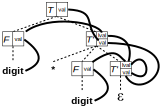
\includegraphics[width=.5\linewidth]{dependency_graph_example2}}
\end{frame}

\sidecite{Knuth.1968}
\begin{frame}{Order of the Attributes}
	\begin{itemize}
	\item The dependency graph characterizes the possible orders in which we can evaluate the attributes at the various nodes of a parse tree.
	\vfill
	\item If the dependency graph has an edge from node $M$ to node $N$, then the attribute corresponding to $M$ must be evaluated before the attribute of $N$.
	\vfill
	\item The only allowable orders of evaluation are those sequences of nodes $N_1, N_2, \dots, N_k$ such that if there is an edge of the dependency graph from $N_i$ to $N_j$, then $i<j$.
	\vfill
	\item Such an ordering embeds a directed graph into a linear order, and is called a topological sort of the graph.
	\end{itemize}
\end{frame}

\sidecite{Knuth.1968, Jazayeri.1975}
\begin{frame}{Problem to Determine the Order of the Attributes}
	\alertbox{If there is any cycle in the graph, then there are no topological sorts; ie. there is no way to evaluate the SDD on the parse tree.}
	\vfill
	\alertbox{Given a SDD, it is very hard to tell whether there exist any parse trees whose dependency graphs have cycles.}
	\vfill
	\begin{itemize}
	\item Translations can be implemented using classes of SDD that guarantee an evaluation order, ie. without cycle.
	\vfill
	\item Two possible approaches to solve this problem:
		\begin{enumerate}
		\item  S-attributed definition.
		\item L-attributed definition.
		\end{enumerate}
	\end{itemize}
\end{frame}

\subsection{S-attributed definition}

\tableofcontentslide[sections={1-4},sectionstyle={show/shaded},subsectionstyle={show/shaded/hide},subsubsectionstyle={show/show/hide/hide}]

\sidecite{Irons.1961}
\begin{frame}{S-Attributed Definition}
	\begin{definition}
		An S-attributed definition is an SDD in which all the attributes are synthesized.
	\end{definition}
	\vspace{4em}
	\begin{itemize}
	\item S-attributed definitions can be implemented during bottom-up parsing, since a bottom-up parse corresponds to a postorder traversal of the parse tree.
	\end{itemize}
\end{frame}

\subsection{L-attributed definition}

\tableofcontentslide[sections={1-4},sectionstyle={show/shaded},subsectionstyle={show/shaded/hide},subsubsectionstyle={show/show/hide/hide}]

\sidecite{Lewis.1974}
\begin{frame}{L-Attributed Definition}
	\begin{footnotesize}
	\begin{definition}
		An L-attributed definition is an SDD in which, between the attributes associated with a production body, dependency-graph edges can go from left to right, but not from right to left.
	\end{definition}
	Each attribute must be:
	\begin{itemize}
	\item Synthesized, or
	\item Inherited, with the rules limited as follows. \\
		Suppose a production \bnftext{A \bnfbody $X_1 X_2 \dots X_n$}, and an inherited attribute $X_i.a$. The rule may uses only:
		\begin{enumerate}[a)]\footnotesize
		\item Inherited attributes associated with the head $A$.
		\item Either inherited or synthesized attributes associated with the occurrences of symbols $X_1 X_2 \dots X_{i-1}$ located to the left of $X_i$.
		\item Inherited or synthesized attributes associated with this occurrence of $X_i$ itself, but only in such a way that there are no cycles in a graph dependency formed by the attributes of this $X$.
		\end{enumerate}
	\end{itemize}
	\end{footnotesize}
\end{frame}

\section{Syntax tree and graph}

\tableofcontentslide[sections={1-6},sectionstyle={show/shaded},subsectionstyle={show/show/hide},subsubsectionstyle={hide/hide/hide/hide}]

\subsection{Syntax tree}

\subsubsection{Definition}

\tableofcontentslide[sections={1-5},sectionstyle={show/shaded},subsectionstyle={show/shaded/hide},subsubsectionstyle={show/show/hide/hide}]

\begin{frame}{Syntax Tree as Intermediate Representation}
	\begin{itemize}
	\item Since some compilers use \emph{syntax tree as an intermediate representation}, a common form of SDD turns its input string into a tree.
	\vfill
	\item To complete the translation to intermediate code, the compiler may then walk the syntax tree, using another set of rules that are in effect an SDD on the syntax tree rather than the parse tree.
	\vfill
	\item Two SDD are considered in this section to build a syntax tree:
		\begin{itemize}
		\item S-attributed definition (bottom-up), and
		\item L-attributed definition (top-down).
		\end{itemize}
	\end{itemize}
\end{frame}

\begin{frame}{Syntax Tree}
	\begin{itemize}
	\item \Emph{Each node in a syntax tree represents a language construct.}
	\item The children of the node represent the meaningful components of the construct.
	\vfill
	\item We shall implement the nodes of a syntax tree by objects with a suitable number of fields.
	\vfill
	\item Each object will have an operator field that is the label of the node, and the following additional fields:
		\begin{itemize}
		\item If the node is a leaf, the lexical value for the leaf.
		\item If the node is an interior node, all the children are stored in individual fields.
		\end{itemize}
	\end{itemize}
\end{frame}

\begin{frame}{Example of a Syntax Tree}
	\begin{center}
		This is the syntax tree for the statement: \\
			\texttt{a := 3 + ( 6 * 7 )} \\[2em]
		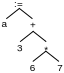
\includegraphics[width=.2\linewidth]{syntax_tree_example2}
	\end{center}
\end{frame}

\subsubsection{Building from S-attributed definition}

\tableofcontentslide[sections={1-5},sectionstyle={show/shaded},subsectionstyle={show/shaded/hide},subsubsectionstyle={show/shaded/hide/hide}]

\begin{frame}[t]{S-Attributed Definition for Building a Syntax Tree}
	\begin{small}
	\begin{center}
		\begin{sdd}[.9\linewidth]
		\p{E ::= E \tok+ T}{head.node = \kw{new} Node(\str{"+"}, E.node, T.node)}
		\p{  ::= E \tok- T}{head.node = \kw{new} Node(\str{"-"}, E.node, T.node)}
		\p{  ::= T}{head.node = T.node}
		\p{T ::= \tok( E \tok)}{head.node = E.node}
		\p{  ::= \tok{id}}{head.node = \kw{new} Leaf(\tok{id}, \tok{id}.lexeme)}
		\p{  ::= \tok{num}}{head.node = \kw{new} Leaf(\tok{num}, \tok{num}.value)}
		\end{sdd}
	\end{center}
	\vspace{2em}
	\begin{itemize}
	\item The semantic rules contain the creation of the syntax tree nodes, with the description of the node and/or the children as parameters. The root of the syntax tree becomes \texttt{E.node}.
	\item Note that the annotated parse tree is implicitly defined by the grammar rules and not directly built by the compiler.
	\end{itemize}
	\end{small}
\end{frame}

\begin{frame}[t]{Example of Syntax Tree Building}
	\begin{small}
	\begin{center}
		\begin{sdd}[.9\linewidth]
		\p{E ::= E \tok+ T}{head.node = \kw{new} Node(\str{"+"}, E.node, T.node)}
		\p{  ::= E \tok- T}{head.node = \kw{new} Node(\str{"-"}, E.node, T.node)}
		\p{  ::= T}{head.node = T.node}
		\p{T ::= \tok( E \tok)}{head.node = E.node}
		\p{  ::= \tok{id}}{head.node = \kw{new} Leaf(\tok{id}, \tok{id}.lexeme)}
		\p{  ::= \tok{num}}{head.node = \kw{new} Leaf(\tok{num}, \tok{num}.value)}
		\end{sdd} \\[1em]
		Input: \texttt{a - 4 + c}
	\end{center}
	\end{small}
	\putat(10,-215){\includeanimatedfigure[height=.4\paperheight]{syntax_tree_sattr}}
	\only<9>{\putat(290,-40){\pgfuseimage{leftarrow}}}
	\only<7>{\putat(290,-50){\pgfuseimage{leftarrow}}}
	\only<5>{\putat(280,-58){\pgfuseimage{leftarrow}}}
	\only<3-4,8>{\putat(270,-79){\pgfuseimage{leftarrow}}}
	\only<6>{\putat(270,-89){\pgfuseimage{leftarrow}}}
\end{frame}

\subsubsection{Building from L-attributed definition}

\tableofcontentslide[sections={1-5},sectionstyle={show/shaded},subsectionstyle={show/shaded/hide},subsubsectionstyle={show/shaded/hide/hide}]

\begin{frame}[t]{L-Attributed Definition for Building a Syntax Tree}
	\begin{small}
	\begin{center}
		\begin{scriptsize}
		\begin{sdd}[.7\linewidth]
		\p{E  ::= T E'}{E'.left = T.node \newl
					head.node = E'.node}
		\p{E' ::= \tok+ T E'}{E'.parent = \kw{new} Node(\str{"+"}, head.left, T.node) \newl
					head.node = E'.node}
		\p{   ::= \tok- T E'}{E'.parent = \kw{new} Node(\str{"-"}, head.left, T.node) \newl
					head.node = E'.node}
		\p{   ::= $\epsilon$}{head.node = head.left}
		\p{T  ::= \tok( E \tok)}{head.node = E.node}
		\p{   ::= \tok{id}}{head.node = \kw{new} Leaf(\tok{id}, \tok{id}.lexeme)}
		\p{   ::= \tok{num}}{head.node = \kw{new} Leaf(\tok{num}, \tok{num}.value)}
		\end{sdd}
		\end{scriptsize}
	\end{center}
	\vspace{2em}
	\begin{itemize}
	\item Note that the annotated parse tree is implicitly defined by the grammar rules and not directly built by the compiler.
	\end{itemize}
	\end{small}
\end{frame}

\begin{frame}[t]{Example of Syntax Tree Building}
	\begin{small}
	\begin{center}
		\begin{scriptsize}
		\begin{sdd}[.7\linewidth]
		\p{E  ::= T E'}{E'.left = T.node \newl
					head.node = E'.node}
		\p{E' ::= \tok+ T E'}{E'.parent = \kw{new} Node(\str{"+"}, head.left, T.node) \newl
					head.node = E'.node}
		\p{   ::= \tok- T E'}{E'.parent = \kw{new} Node(\str{"-"}, head.left, T.node) \newl
					head.node = E'.node}
		\p{   ::= $\epsilon$}{head.node = head.left}
		\p{T  ::= \tok( E \tok)}{head.node = E.node}
		\p{   ::= \tok{id}}{head.node = \kw{new} Leaf(\tok{id}, \tok{id}.lexeme)}
		\p{   ::= \tok{num}}{head.node = \kw{new} Leaf(\tok{num}, \tok{num}.value)}
		\end{sdd}
		\end{scriptsize}\\[1em]
		Input: \texttt{a - 4 + c}
	\end{center}
	\end{small}
	\putat(-10,-215){\includeanimatedfigure[height=.35\paperheight]{syntax_tree_lattr}}
	\only<5>{\putat(258,-39){\pgfuseimage{leftarrow}}}
	\only<13>{\putat(258,-46){\pgfuseimage{leftarrow}}}
	\only<9>{\putat(258,-53){\pgfuseimage{leftarrow}}}
	\only<11>{\putat(258,-59){\pgfuseimage{leftarrow}}}
	\only<7>{\putat(258,-67){\pgfuseimage{leftarrow}}}
	\only<12>{\putat(258,-73){\pgfuseimage{leftarrow}}}
	\only<10>{\putat(258,-81){\pgfuseimage{leftarrow}}}
	\only<4,8>{\putat(258,-94){\pgfuseimage{leftarrow}}}
	\only<6>{\putat(258,-102){\pgfuseimage{leftarrow}}}
\end{frame}

\subsection{Directed acyclic graph}

\tableofcontentslide[sections={1-6},sectionstyle={show/shaded},subsectionstyle={show/shaded/hide},subsubsectionstyle={show/show/hide/hide}]

\begin{frame}{Directed Acyclic Graph}
	\begin{itemize}
	\item Nodes in a syntax tree represent language constructs in the source program; the children of a node represent the meaningful components of a construct.
	\end{itemize}
	\vfill
	\begin{definition}[Directed Acyclic Graph]
		A directed acyclic graph (DAG) represent the language constructs un the source program.
		It ensures that a construct is present only one time in the DAG.
	\end{definition}
	\vfill
	\begin{itemize}
	\item The difference between syntax tree and DAG is that the DAG node may have more than one parent.
	\item Consequently, a subexpression is repeated in a tree; and shared in a DAG.
	\end{itemize}
\end{frame}

\begin{frame}{Example of Directed Acyclic Graph}
	\begin{center}
		$a \tok+ a \tok* \tok( b \tok- c \tok) \tok+ \tok( b \tok- c \tok) \tok* d$
	\end{center}
	\vspace{2em}
	\includeanimatedfigure[width=\linewidth]{dag_example}
\end{frame}

\begin{frame}[fragile]{Value-Number Representation for the DAG}
	\begin{footnotesize}
	\begin{itemize}
	\item Often, the nodes of a DAG are stored in an array of records (also true for a syntax tree).
	\end{itemize}
	\begin{columns}
		\begin{column}{.2\linewidth}
			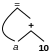
\includegraphics[width=\linewidth]{simple_dag}
		\end{column}
		\begin{column}{.4\linewidth}
			\begin{scriptsize}
			\begin{tabularx}{\linewidth}{|c|X|X|X|}
				\hline
				1 & \tok{id} & \multicolumn{2}{l|}{to symbol $a$} \\
				\hline
				2 & \tok{num} & \multicolumn{2}{l|}{10} \\
				\hline
				3 & \tok+ & 1 & 2 \\
				\hline
				4 & \tok= & 1 & 3 \\
				\hline
			\end{tabularx}
			\end{scriptsize}
		\end{column}
		\begin{column}{.4\linewidth}
			\begin{scriptsize}
			\begin{lstlisting}[language=C]
			struct {
			   int token_id;
			   union {
			      unsigned int symbol_index;
			      double fvalue;
			      long lvalue;
			      struct {
			         unsigned int left;
			         unsigned int right;
			      } operands;
			   } attr;
			} Record;
			\end{lstlisting}
			\end{scriptsize}
		\end{column}
	\end{columns}
	\begin{itemize}
	\item Each node of the DAG is referred by its index in the table; its \emph{value number}.
	\item Let the signature of an interior node be the triple $\langle op,l,r \rangle$, where $op$ is the label, $l$ its left child's value number, and $r$ its right child's value number. $l$ and $r$ are set to $0$ when there is no child.
	\end{itemize}
	\end{footnotesize}
\end{frame}

\begin{frame}[fragile]{Building a DAG}
	\begin{description}
	\item[INPUT] Label $op$, node $l$, and node $r$.
	\item[OUTPUT] The value number of a node in the array with signature $\langle op,l,r \rangle$.
	\vfill
	\item[METHOD] Search the array for a node $M$ with label $op$, left child $l$, and right child $r$. If there is such a node return the value number of $M$. If not, create in the array a new node $N$ with label $op$, left child $l$, right child $r$, and return its value number.
	\vfill
	\item[NOTE] This approach is searching the entire array every time; it is not efficient. A more efficient approach is to use a hash table, in which the nodes are put into ``buckets,'' each of which typically will have only few nodes.
	\end{description}
\end{frame}

\section{Three-address code}

\tableofcontentslide[sections={1-5},sectionstyle={show/shaded},subsectionstyle={show/show/hide},subsubsectionstyle={hide/hide/hide/hide}]

\sidecite{Strong.1958, Wirth.1971, Johnson.1979, Ritchie.1979}
\begin{frame}{Level of Intermediate Representation}
	\alertbox*{The syntax tree is a \Emph{high-level} intermediate representation of the source program.}
	\vspace{2em}
	\alertbox{To make easier the generation of low-level code, a low-level intermediate representation is useful.}
	\vspace{2em}
	\alertbox*{The \Emph{three-address code} is a form of low-level intermediate representation that is close to the assembler languages.}
	\begin{tiny}
		\alert{Note:} The rest of this lecture focuses on the generation of code with three-address code. The syntax tree may be also used as a basis of the generation (see the supervised tutorials).
	\end{tiny}
\end{frame}

\sidecite{Strong.1958, Gosling.1995}
\begin{frame}{What is Three-Address Code?}
	\begin{itemize}
	\item In three-address code, there is at most one operator on the right side of an instruction.
		\begin{center}
			\begin{tac}[.3\linewidth]
				\a{\t1}{y * z}
				\a{\t2}{x + \t2}
			\end{tac}
		\end{center}
	\item where \tactext{\t1} and \tactext{\t2} are  compiler-generated temporary names.
	\end{itemize}
	\begin{columns}
		\begin{column}{.3\linewidth}
			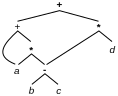
\includegraphics[width=\linewidth]{dag_alone_example}
		\end{column}
		\begin{column}{.5\linewidth}
			\begin{tac}[\linewidth]
				\a{\t1}{b - c}
				\a{\t2}{a * \t1}
				\a{\t3}{a + \t2}
				\a{\t4}{\t1 * d}
				\a{\t5}{\t3 + \t4}
			\end{tac}
		\end{column}
	\end{columns}
\end{frame}

\subsection{Language basics}

\begin{frame}{Address}
	An address can be one of the following:
	\begin{enumerate}
	\item[Name] For convenience, we allow source-program names to appear as addresses in three-address code. In an implementation, a source name is replaced by a pointer to its symbol-table entry, where all information about the name is kept.
	\vfill
	\item[Constant] A compiler must deal with many different types of constants and variables.
	\vfill
	\item[Compiler-generated temporary Name] It is useful, especially in optimizing compilers, to create a distinct name each time a temporary is needed. These temporaries can be combined, if possible, when registers are allocated to variables.
	\end{enumerate}
\end{frame}

\begin{frame}{Label}
	\begin{itemize}
	\item A symbolic label represents the index of a three-address instruction in the sequence of instructions.
	\item Numeric positions can be substituted for the labels, either by making a separate pass or by ``backpatching.''
	\end{itemize}
	\begin{columns}
		\begin{column}{.4\linewidth}
			\begin{center}
			\begin{tac}[\linewidth]
				\a[L]{\t1}{i + 1}
				\a{i}{\t1}
				\a{\t2}{i * 8}
				\a{\t3}{a [ \t2 ]}
				\ifgoto{\t3 $<$ v}{L}
			\end{tac} \\[1em]
			\emph{Symbolic Label}
			\end{center}
		\end{column}
		\begin{column}{.5\linewidth}
			\begin{center}
			\begin{tac}[\linewidth]
				\a[103]{\t1}{i + 1}
				\a[104]{i}{\t1}
				\a[105]{\t2}{i * 8}
				\a[106]{\t3}{a [ \t2 ]}
				\ifgoto[107]{\t3 $<$ v}{103}
			\end{tac} \\[1em]
			\emph{Numeric Position}
			\end{center}
		\end{column}
	\end{columns}
\end{frame}

\begin{frame}{Assignment Instruction}
	\begin{itemize}
	\item Assignment instruction of the form \emph{\tactext{x = y {\textless}op{\textgreater} z}}, where \tactext{{\textless}op{\textgreater}} is a binary arithmetic or logical operation, and \tactext{x}, \tactext{y}, and \tactext{z} are addresses.
	\vfill
	\item Assignment instruction of the form \emph{\tactext{x = {\textless}op{\textgreater} y}}, where \tactext{{\textless}op{\textgreater}} is an unary operation. Essential unary operations include unary minus, logical negation, and conversion operators.
	\vfill
	\item Copy instruction of the form \emph{\tactext{x = y}}, where \tactext{x} is assigned the value of \tactext{y}.
	\end{itemize}
\end{frame}

\begin{frame}{Jumping Instruction}
	\begin{itemize}
	\item An unconditional jump \emph{\tactext{\kw{goto} L}}. The three-address instruction with label \tactext{L} is the next executed.
	\vfill
	\item Conditional jumps of the form \emph{\tactext{\kw{if} x \kw{goto} L}}, and \emph{\tactext{\kw{ifFalse} x \kw{goto} L}}. These instructions execute the instruction with label \tactext{L} next if \tactext{x} is true and false, respectively. Otherwise, the following three-address instruction in sequence is executed next, as usual.
	\vfill
	\item Conditional jumps such as \emph{\tactext{\kw{if} x {\textless}relop{\textgreater} y \kw{goto} L}}, which apply a relational operator ($<$, $<=$, $>$\dots) to \tactext{x} and \tactext{y}, and execute the instruction with label \tactext{L} next if \tactext{x} stands in relation \tactext{{\textless}relop{\textgreater}} to \tactext{y}. If not, the following three-address instruction in sequence is executed next.
	\end{itemize}
\end{frame}

\begin{frame}{Procedure Call Instruction}
	\begin{columns}
		\begin{column}{.8\linewidth}
		\begin{small}
		Procedure calls and returns are implemented using the following instructions:
		\vfill
		\begin{itemize}
		\item \tactext{\kw{param} x} for passing values as parameters
		\vfill
		\item \tactext{\kw{call} p,n} for the procedure call
		\vfill
		\item \tactext{y = \kw{call} p,n} for the function call
		\vfill
		\item \tactext{\kw{return} y} for returning a value.
		\end{itemize}
		\vfill
		where \tactext{x} and \tactext{y} are addresses, \tactext{p} is the name of the subroutine, \tactext{n} is the number of parameters to pass to the subroutine.
		\end{small}
		\end{column}
		\begin{column}{.2\linewidth}
			\begin{tac}[\linewidth]
				\param{x$_1$}
				\param{x$_2$}
				\tacdots
				\param{x$_n$}
				\callproc{p,n}
			\end{tac}
		\end{column}
	\end{columns}
	\vfill
	\alertbox{Procedures and their implementation are detailled in Chapter~\ref{chap:runtime_environments}.}
\end{frame}

\begin{frame}{Index Copy Instruction}
	\begin{itemize}
	\item Indexed copy instruction has one of the forms:
		\begin{itemize}
		\item \emph{\tactext{x = y[i]}}
		\item \emph{\tactext{x[i] = y}}
		\end{itemize}
	\vfill
	\item The first instruction form sets \tactext{x} to the value of the i$^{\text{th}}$ memory unit beyond \tactext{y}.
	\vfill
	\item The second instruction form sets the contents of the i$^{\text{th}}$ unit beyond \tactext{x} to the value of \tactext{y}.
	\end{itemize}
\end{frame}

\begin{frame}{Address and Pointer Assignment Instruction}
	Address and pointer assignment has one of the forms:
	\vfill
	\begin{itemize}
	\item \emph{\tactext{x = \&y}}: sets \tactext{x} to the location of \tactext{y}.
	\vfill
	\item \emph{\tactext{x = *y}}: sets \tactext{x} to the value of the variable at the memory address \tactext{y}.
	\vfill
	\item \emph{\tactext{*x = y}}: sets the variable at the memory address \tactext{x} to the value of \tactext{y}.
	\end{itemize}
\end{frame}

\begin{frame}{Example of Three-Adress Code}
	\begin{itemize}
	\item Consider the statement:
		\begin{center}
			\code{\kw{do} i = i + 1; \kw{while} (a[i] $<$ v);}
		\end{center}
	\item The translation is three-address code is the following, assuming that the type of the elements of "a" takes 8 units of memory each.
	\end{itemize}
	\begin{center}
	\begin{tac}[.5\linewidth]
		\a[L]{\t1}{i + 1}
		\a{i}{\t1}
		\a{\t2}{i * 8}
		\a{\t3}{a[\t1]}
		\ifgoto{\t2 $<$ v}{L}
	\end{tac}
	\end{center}
\end{frame}

\begin{frame}{Other Three-Address Operations?}
	\begin{itemize}
	\item The choice of allowable operators is an important issue in the design of an intermediate form.
	\vfill
	\item The operator set clearly must be rich enough to implement  the operations from the source language.
	\vfill
	\item Operators that are close to machine instructions make it easier to implement the intermediate form on a target machine.
	\vfill
	\item However, if the front end must generate long sequences of instructions for some source-language operations, then the optimizer and code generator may have to work harder to rediscover the structure and generate good code for these operations.
	\end{itemize}
\end{frame}

\begin{frame}{Implementation of Three-Address Code}
	\alertbox*{Three-address instructions could be implemented in a compiler as objects or as records.}
	\vspace{3em}
	\alertbox{Three representations are commonly used: \\ quadruple, triples, and indirect triples.}
\end{frame}

\subsection{Quadruple form}

\tableofcontentslide[sections={1-5},sectionstyle={show/shaded},subsectionstyle={show/shaded/hide},subsubsectionstyle={show/show/hide/hide}]

\begin{frame}{Quadruple Form}
	\begin{itemize}
	\item A quadruple has four fields: 
		\begin{center}
			\tactext{{\textless}op{\textgreater} {\textless}arg$_1${\textgreater} {\textless}arg$_2${\textgreater} {\textless}result{\textgreater}}
		\end{center}
	\vfill
	\item \tactext{{\textless}op{\textgreater}}: this field contains an internal code for the operator.
	\item \tactext{{\textless}arg$_1${\textgreater}} and \tactext{{\textless}arg$_2${\textgreater}}: they are the arguments of the operator.
	\item \tactext{{\textless}result{\textgreater}}: it contains the result value computed by the operator.
	\end{itemize}
\end{frame}

\begin{frame}{Example of Quadruples}
	\begin{columns}
		\begin{column}{.5\linewidth}
			\begin{tac}[\linewidth]
				\a{\t1}{minus c}
				\a{\t2}{b * \t1}
				\a{\t3}{minus c}
				\a{\t4}{b * \t3}
				\a{\t5}{\t2 + \t4}
				\a{a}{\t5}
			\end{tac}
		\end{column}
		\begin{column}{.5\linewidth}
			\begin{tabularx}{\linewidth}{|X|X|X|X|}
			\hline
			\tabularheading\chead{op}&\chead{arg$_1$}&\chead{arg$_2$}&\chead{result}\\
			\hline
			minus & c & & \tactext{t$_1$} \\
			\hline
			* & b & \tactext{t$_1$} & \tactext{t$_2$} \\
			\hline
			minus & c & & \tactext{t$_3$} \\
			\hline
			* & b & \tactext{t$_3$} & \tactext{t$_4$} \\
			\hline
			+ & \tactext{t$_2$} & \tactext{t$_4$} & \tactext{t$_5$} \\
			\hline
			= & \tactext{t$_5$} & & \tactext{a} \\
			\hline
			\end{tabularx}
		\end{column}
	\end{columns}
\end{frame}

\begin{frame}[fragile]{Example of Implementation in C}
	\begin{lstlisting}[language=C,basicstyle=\scriptsize]
	/* Operations supported by the three-address code */
	typedef enum { MULTIPLY, ADD, MINUS, ...} Operator;

	/* Definition of a parameter or a return value */
	typedef union { 
	   unsigned long address; /* address of a variable */
	   long integer_value;    /* integer constant */
	   double float_value;    /* floating-point constant */
	} Value;

	/* Definition of a single quadruple */
	typedef struct {
	   Operator operator;
	   Value arg1;
	   Value arg2;
	   Value result;
	} Quadruple;
	\end{lstlisting}
\end{frame}

\subsection{Triple form}

\tableofcontentslide[sections={1-5},sectionstyle={show/shaded},subsectionstyle={show/shaded/hide},subsubsectionstyle={show/show/hide/hide}]

\begin{frame}{Triple Form}
	\begin{itemize}
	\item A triple has only three fields:
		\begin{center}
			\tactext{{\textless}op{\textgreater} {\textless}arg$_1${\textgreater} {\textless}arg$_2${\textgreater}}
		\end{center}
	\vfill
	\item Note that result in quadruples is primarily used for temporary names. 
	\item The result of an operation \tactext{x {\textless}op{\textgreater} y} is refered by its position, rather than by an explicit temporary name.
	\item Thus instead of the temporary \tactext{t$_1$} in the previous example, a triple representation would refer to position \tactext{(0)}.
	\item Parenthesized numbers represent points into the triple structure itself.
	\end{itemize}
\end{frame}

\begin{frame}{Example of Triples}
	\begin{columns}
		\begin{column}{.5\linewidth}
			\begin{tac}[\linewidth]
				\a{\t1}{minus c}
				\a{\t2}{b * \t1}
				\a{\t3}{minus c}
				\a{\t4}{b * \t3}
				\a{\t5}{\t2 + \t4}
				\a{a}{\t5}
			\end{tac}
		\end{column}
		\begin{column}{.5\linewidth}
			\begin{tabularx}{\linewidth}{|c|X|X|X|}
			\hline
			\tabularheading&\chead{op}&\chead{arg$_1$}&\chead{arg$_2$}\\
			\hline
			0 & minus & c & \\
			\hline
			1 & * & b & (0) \\
			\hline
			2 & minus & c & \\
			\hline
			3 & * & b & (2) \\
			\hline
			4 & + & (1) & (3) \\
			\hline
			5 & = & \tactext{a} & (4) \\
			\hline
			\end{tabularx}
		\end{column}
	\end{columns}
\end{frame}

\begin{frame}[fragile]{Example of Implementation in C}
	\begin{lstlisting}[language=C,basicstyle=\scriptsize]
	/* Operations supported by the three-address code */
	typedef enum { MULTIPLY, ADD, MINUS, ...} Operator;

	/* Definition of a parameter or a return value */
	typedef union { 
	   unsigned long address; /* address of a variable */
	   long integer_value;    /* integer constant */
	   double float_value;    /* floating-point constant */
	} Value;

	/* Definition of a single triple */
	typedef struct {
	   Operator operator;
	   Value arg1;
	   Value arg2;
	} Triple;
	\end{lstlisting}
\end{frame}


\begin{frame}{Why Quadruple or Triple?}
	\begin{itemize}
	\item A benefit of quadruples over triples can be seen in an optimizing compiler, where instructions are often moved around.
	\vfill
	\item With quadruples, if we move an instruction that computes a temporary \tactext{t}, then the instructions that use \tactext{t} require no change.
	\vfill
	\item With triples, the result of an operation is referred to by its position, so moving an instruction may require us to change all references to that result.
	\end{itemize}
	\vfill
	\alertbox*{This problem does not occur with indirect triples.}
\end{frame}

\begin{frame}{Indirect Triple}
	\begin{small}
	\begin{itemize}
	\item Indirect triples consist of a listing of points to triples, rather than a listing of triples themselves.
	\item With indirect triples, an optimizing compiler can move an instruction by reordering the instruction list, without affecting the triples themselves.
	\end{itemize}
	\begin{columns}
		\begin{column}{.5\linewidth}
			\begin{center}
			\begin{tabular}{|c|c|}
			\hline
			35 & (0) \\
			36 & (1) \\
			37 & (2) \\
			38 & (3) \\
			39 & (4) \\
			40 & (5) \\
			\hline
			\end{tabular}
			\end{center}
		\end{column}
		\begin{column}{.5\linewidth}
			\begin{tabularx}{\linewidth}{|c|X|X|X|}
			\hline
			\tabularheading&\chead{op}&\chead{arg$_1$}&\chead{arg$_2$}\\
			\hline
			0 & minus & c & \\
			\hline
			1 & * & b & (0) \\
			\hline
			2 & minus & c & \\
			\hline
			3 & * & b & (2) \\
			\hline
			4 & + & (1) & (3) \\
			\hline
			5 & = & \tactext{a} & (4) \\
			\hline
			\end{tabularx}
		\end{column}
	\end{columns}
	\begin{itemize}
	\item When implemented in Java, an array of instruction objects is analogous to an indirect triple representation, since Java treats the array elements as references to objects.
	\end{itemize}
	\end{small}
\end{frame}

\subsection{Static single-assignment form}

\tableofcontentslide[sections={1-5},sectionstyle={show/shaded},subsectionstyle={show/shaded/hide},subsubsectionstyle={show/show/hide/hide}]

\begin{frame}{Static-Single Assignement Form}
	\begin{definition}
		Static single-assignment form (SSA) is an intermediate representation that facilitates certain code optimizations.
	\end{definition}
	\vspace{3em}
	Two distinctive aspects distinguish SSA from the standard form of the three-address code.
	\begin{enumerate}
	\item All assignments in SSA are to variables with distinct names.
	\item Introduction of the $\phi$-function.
	\end{enumerate}
\end{frame}

\begin{frame}{Distinct Assignements in SSA}
	\begin{itemize}
	\item All assignments in SSA are to variables with distinct names.
	\end{itemize}
	\vspace{2em}
	\begin{columns}
		\begin{column}{.5\linewidth}
			\begin{center}
			\begin{tac}[\linewidth]
				\a{p}{a + b}
				\a{q}{p - c}
				\a{p}{q * d}
				\a{p}{e - p}
				\a{q}{p + q}
			\end{tac}
			\vspace{1em}
			Standard Form
			\end{center}
		\end{column}
		\begin{column}{.5\linewidth}
			\begin{center}
			\begin{tac}[\linewidth]
				\a{p$_1$}{a + b}
				\a{q$_1$}{p$_1$ - c}
				\a{p$_2$}{q$_1$ * d}
				\a{p$_3$}{e - p$_2$}
				\a{q$_2$}{p$_3$ + q$_1$}
			\end{tac}
			\vspace{1em}
			SSA Form
			\end{center}
		\end{column}
	\end{columns}
\end{frame}

\begin{frame}{$\phi$-Function}
	\begin{itemize}
	\item A notational convention, called $\phi$-function, is introduced to combine two definitions of the same variable in parallel control-flow paths.
	\item For example, the source program:
		\begin{myalgorithm}
			\lIf{flag}{x = -1}\;
			\lElse{x = 1}\;
			y = x * a\;
		\end{myalgorithm}
	\item has two control-flow paths in which the variable \tactext{x} is defined. It is impossible to known which of the two \tactext{x} is used in \tactext{x * a}.
	\item We introduce the $\phi$-function that replies the ``defined'' value:
		\begin{myalgorithm}
			\lIf{flag}{x$_1$ = -1}\;
			\lElse{x$_2$ = 1}\;
			y = $\phi$(x$_1$, x$_2$) * a\;
		\end{myalgorithm}
	\end{itemize}
\end{frame}

\section[Generation of variables]{Code generation of variables}

\tableofcontentslide[sections={2-6},sectionstyle={show/shaded},subsectionstyle={show/show/hide},subsubsectionstyle={hide/hide/hide/hide}]

\subsection{Types and declarations}

\subsubsection{Introduction}

\tableofcontentslide[sections={2-6},sectionstyle={show/shaded},subsectionstyle={show/shaded/hide},subsubsectionstyle={show/show/hide/hide}]

\begin{frame}{Types and Declarations}
	The application of types can be grouped as follows:
	\vfill
	\begin{enumerate}
	\item[Type checking] It uses logical rules to reason about the behavior of a program at runtime. Specifically, it ensures that the types of the operands match the type expected by an operator.
	\vfill
	\item[Translation applications] From the type of a name, a compiler can determine the storage that will be needed for that name at runtime. Type information is also needed to calculate the address denoted by an array reference, to insert explicit type conversions, and to choose the right version of an arithmetic operator\dots
	\end{enumerate}
\end{frame}

\subsubsection{Type descriptions}

\tableofcontentslide[sections={3-6},sectionstyle={show/shaded},subsectionstyle={show/shaded/hide},subsubsectionstyle={show/shaded/hide/hide}]

\begin{frame}{Type Expressions}
	\begin{itemize}
	\item \emph{Types have structure represented by the type expressions.}
	\vfill
	\item A type expression is either a basic type or is formed by applying an operator called a type constructor to a type expression.
	\vfill
	\item The set of basic types and constructors depend on the language to be checked.
	\end{itemize}
\end{frame}

\begin{frame}{What is a Type Expression?}
	\begin{enumerate}
	\item \emph{Basic type}: \kw{boolean}, \kw{char}, \kw{integer}, \kw{float}, \kw{void}.
	\item \emph{Type name}.
	\item Expression built with the \emph{array type constructor}.
	\item \emph{Record}: data structure with named fields.
	\item \emph{Function prototype}: by using the function prototype constructor $inputType \rightarrow outputType$.
	\item \emph{Cartesian product} of two type expressions: if $s$ and $t$ are type expressions, then $s \times t$ is a type expression.
	\end{enumerate}
\end{frame}

\subsubsection{Type equivalence}

\tableofcontentslide[sections={3-6},sectionstyle={show/shaded},subsectionstyle={show/shaded/hide},subsubsectionstyle={show/shaded/hide/hide}]

\begin{frame}[b]{Type Equivalence}
	\begin{footnotesize}
	\alertbox{We must define how to convert a value from one type to others. Many type-checking rules have the form, ``if two type expressions are equal then return a certain type else error.''}
	\begin{definition}[Type Equivalence]\small
		Two types are structurally equivalent when:
		\begin{enumerate}
		\item\label{def:type:equivalence:a}They are the same basic type.
		\item\label{def:type:equivalence:b}They are formed by applying the same constructor to structurally equivalent types.
		\item One is a type name that denotes the other.
		\end{enumerate}
	\end{definition}
	\begin{itemize}
	\item Points \ref{def:type:equivalence:a} and \ref{def:type:equivalence:b} are used to defined the equivalence between two type names, ie. the name equivalence.
	\end{itemize}
	\end{footnotesize}
\end{frame}

\subsubsection{Declarations}

\tableofcontentslide[sections={3-6},sectionstyle={show/shaded},subsectionstyle={show/shaded/hide},subsubsectionstyle={show/shaded/hide/hide}]

\begin{frame}{Declarations}
	\begin{itemize}
	\item Declaration of types is handled by a grammar like:
		\begin{center}
		\begin{bnf}[.6\linewidth]
		\p{D ::= T \tok{id} \tok; D}
		\p{  ::= $\epsilon$}
		\p{T ::= B C}
		\p{  ::= \tok{record} \tok\{ D \tok\}}
		\p{B ::= \tok{int} \bnfor \tok{float}}
		\p{C ::= \tok[ \tok{num} \tok] C}
		\p{  ::= $\epsilon$}
		\end{bnf}
		\end{center}
	\item This grammar supports basic types, arrays and records.
		\begin{itemize}
		\item \kw{float};
		\item \kw{int}[3][4];
		\item \kw{record} \{ \kw{float} name1; \kw{record} \{ \kw{int} name2; \} \}
		\end{itemize}
	\end{itemize}
\end{frame}

\subsubsection{Storage layout for local names}

\tableofcontentslide[sections={3-6},sectionstyle={show/shaded},subsectionstyle={show/shaded/hide},subsubsectionstyle={show/shaded/hide/hide}]

\begin{frame}{Storage Layout for the Local Names}
	\begin{itemize}
	\item \emph{From the type of a name, we can determine the amount of storage that will be needed for the name at runtime.}
	\vfill
	\item At compile time, we can use these amounts to assign each name a relative address.
	\vfill
	\item Both the type and relative address are saved in the symbol table.
	\vfill
	\item Data of varying length (string, dynamic array\dots) is handled by reserving a known fixed amount of storage for a pointer to the data.
	\item Runtime storage management is not discussed in this chapter, but in the chapter~\ref{chap:runtime_environments}.
	\end{itemize}
\end{frame}

\begin{frame}{Size of the Names}
	\begin{itemize}
	\item Data of varying length (string, dynamic array\dots) is handled by reserving a known fixed amount of storage for a pointer to the data.
	\vfill
	\item The \emph{width of a type} (and not of a variable) is the number of storage units (usually bytes) needed for objects of that type.
	\vfill
	\item A basic type requires an integral number of storage units.
	\vfill
	\item For easy access, storage for aggregates such as arrays and classes is allocated in one contiguous block of storage units.
	\end{itemize}
\end{frame}

\begin{frame}[b]{Address Alignement}
	\begin{footnotesize}
	\alertbox{The storage layout for data objects is strongly influenced by the addressing constraints of the target machine.}
	\begin{examples}
		\begin{itemize}
		\item Instructions to add integers may expect integers to be aligned, ie. placed at certain positions in memory such as an address divisible by 4.
		\item An array of ten characters needs only enough bytes to hold ten characters, a compiler may therefore allocate 12 bytes (the next multiple of 4).
		\end{itemize}
	\end{examples}
	\begin{itemize}
	\item  Space left unused due to alignment considerations is referred to as padding.
	\item \emph{A compiler may pack data so that no padding is left}; additional instructions may then need to be executed at runtime to position packed data so that it can be operated on as if it were properly assigned.
	\end{itemize}
	\end{footnotesize}
\end{frame}

\begin{frame}{Determine the Type and its Width}
	\begin{itemize}
	\item The SDT below computes types and their widths for basic and array types. Records will be discussed later.
		\begin{sdd}[\linewidth]
		\p{T ::= B}{t = B.type; w = B.width}
		\p{  ::= C}{T.type = C.type; T.width = C.width}
		\p{B ::= \tok{int}}{B.type = integer; B.width = 4}
		\p{  ::= \tok{float}}{ B.type = float; B.width = 8}
		\p{C ::= \tok{[} \tok{num} \tok{]} C}{head.type = \kw{array}(num.value,C.type); \newl
						  head.width = num.value * C.width;}
		\p{  ::= $\epsilon$}{head.type = t; head.width = w;}
		\end{sdd}
		\vfill
	\item The SDT uses synthesized attributes type and width for each nonterminal and two variable $t$ and $w$ to pass type and width information from a $B$ node in a parse tree to the node for the production \bnftext{C \bnfbody $\epsilon$}.
	\item In a syntax-directed definition, $t$ and $w$ would be inherited attributes for $C$.
	\end{itemize}
\end{frame}

\subsubsection{Sequence of declarations}

\tableofcontentslide[sections={3-6},sectionstyle={show/shaded},subsectionstyle={show/shaded/hide},subsubsectionstyle={show/shaded/hide/hide}]

\begin{frame}{Sequence of Declarations}
	\begin{itemize}
	\item Modern languages allow all the declarations in a single procedure to be processed as a group.
	\vfill
	\item The declarations may be distributed within a procedure \eg in Java, but they can still be processed when the procedure is analyzed.
	\vfill
	\item We use a variable, say offset, to keep track of the next available relative address.
	\end{itemize}
\end{frame}

\begin{frame}{Definition of a Sequence of Declarations}
	\begin{itemize}
	\item The following SDT illustrates the use of \emph{offset}:
		\begin{sdd}
		\p{P ::=}{offset = 0}
		\pcont{D}{}
		\p{D ::= T \tok{id}}{	s = \kw{new} Symbol(\tok{id}.lexeme) \newl
					s.offset = offset ; s.type = T.type \newl
					SymbolTable.getCurrent().declare(\tok{id}.lexeme, s) \newl
					offset = offset + T.width;}
		\pcont{D}{}
		\p{  ::= $\epsilon$}{}
		\end{sdd}
		\vfill
	\item The semantic action associated to the head $D$ creates a symbol table entry.
	\item The symbol table takes the name of the variable (its lexeme), the type of the variable, and the position of the variable in the storage.
	\end{itemize}
\end{frame}

\subsubsection{Fields in record or class}

\tableofcontentslide[sections={3-6},sectionstyle={show/shaded},subsectionstyle={show/shaded/hide},subsubsectionstyle={show/shaded/hide/hide}]

\begin{frame}{Definition of Records or Classes}
	\begin{itemize}
	\item The previous sequence of declarations may be used to define the fields in records and classes.
	\item We may extend the previous grammar with the $T$-production.
		\begin{sdd}
		\p{T ::= B}{t = B.type, w = B.width}
		\pcont{C}{T.type = C.type; T.width = C.width}
		\p{  ::= \tok{record} \tok{\{} T \tok{\}}}{}
		\p{B ::= \tok{int}}{B.type = integer; B.width = 4}
		\p{  ::= \tok{float}}{B.type = float; B.width = 8}
		\p{C ::= \tok{[} \tok{num} \tok{]} C}{head.type = \kw{array}(num.value,C.type) \newl
				head.width = num.value * C.width}
		\p{  ::= $\epsilon$}{head.type = t; head.width = w}
		\end{sdd}
		\vfill
	\item The field names in a record must be distinct.
	\item The offset or relative address for a field name is relative to the data area for that record.
	\end{itemize}
\end{frame}

\begin{frame}{Define an Environment for Each Record}
	\begin{itemize}
	\item For convenience, the record is defined with a specific symbol table, or environment.
		\begin{sdd}
		\p{T ::= \tok{record} \tok{\{}}{
					SymbolTable.getCurrent().offset = offset; \newl
					SymbolTable.openContext(); \newl
					offset = 0;}
		\pcont{T \tok{\}}}{	T.type = \kw{record}(SymbolTable.getCurrent()); \newl
					T.width = offset; \newl
					SymbolTable.closeContext(); \newl
					offset = SymbolTable.getCurrent().offset;}
		\end{sdd}
		\vfill
	\item The SDT may be updated as above, where \code{SymbolTable} is defined in chapter~\ref{chap:overview}.
	\item \emph{Classes are stored as records, since no storage is reserved for methods.}
	\end{itemize}
\end{frame}

\subsection{Expressions}

\subsubsection{Introduction}

\tableofcontentslide[sections={3-6},sectionstyle={show/shaded},subsectionstyle={show/shaded/hide},subsubsectionstyle={show/show/hide/hide}]

\begin{frame}{Translation of Expressions}
	\begin{itemize}
	\item \emph{This section describes how the expressions are translated into three-address code.}
	\vfill
	\item An expression with more than one operator, like \code{a+b*c}, will translate into instructions with at most one operator per instruction.
	\item An array reference $A[i][j]$ will expand into a sequence of three-address instructions that calculate an address for the reference.
	\vfill
	\item The translation function may be placed in two locations:
		\begin{enumerate}
		\item inside the semantic actions themselves; or
		\item inside a dedicated method, usually called \texttt{generate()}, of the syntax tree.
		\end{enumerate}
	\end{itemize}
\end{frame}

\subsubsection{Operations within expressions}

\tableofcontentslide[sections={3-6},sectionstyle={show/shaded},subsectionstyle={show/shaded/hide},subsubsectionstyle={show/shaded/hide/hide}]

\begin{frame}[t]{Translation of the Expressions}
	\begin{itemize}
	\item Each operation in the expression are translated to its equivalent three-address code.
	\item The SDT below builds up the three-address code for the assignment and several arithmetic operations.
	\end{itemize}
	\putat(-10,-150){\parbox{.9\paperwidth}{\mdseries\normalcolor\footnotesize
	\begin{sdd}
	\p{S ::= \tok{id} \tok= E \tok;}{head.code = E.code \concat quadruple(\str{'='}, E.addr, \newl \hspace{1em}$\emptyset$, SymbolTable.getCurrent().get(\tok{id}.lexeme))}
	\p{E ::= E \tok+ E}{head.addr = \kw{new} TemporaryVariable(); \newl head.code = E$_1$.code \concat E$_2$.code \concat \newl quadruple(\str{'+'}, E$_1$.addr, E$_2$.addr, head.addr)}
	\p{E ::= \tok- E}{head.addr = \kw{new} TemporaryVariable(); \newl head.code = E.code \concat \newl quadruple(\str{'minus'}, E.addr, $\emptyset$, head.addr)}
	\p{  ::= \tok( E \tok)}{head.addr = E.addr; head.code = E.code}
	\p{  ::= \tok{id}}{head.addr = SymbolTable.getCurrent().get(\tok{id}.lexeme) \newl head.code = ''}
	\end{sdd}
	}}
\end{frame}

\begin{frame}[t]{Concatenation Operator}
	\begin{itemize}
	\item The operator \emph{\code{\concat}} denotes the concatenation of strings of characters.
	\end{itemize}
	\putat(-10,-150){\parbox{.9\paperwidth}{\mdseries\normalcolor\footnotesize
	\begin{sdd}
	\p{S ::= \tok{id} \tok= E \tok;}{head.code = E.code \alertconcat quadruple(\str{'='}, E.addr, \newl \hspace{1em}$\emptyset$, SymbolTable.getCurrent().get(\tok{id}.lexeme))}
	\p{E ::= E \tok+ E}{head.addr = \kw{new} TemporaryVariable(); \newl head.code = E$_1$.code \alertconcat E$_2$.code \alertconcat \newl quadruple(\str{'+'}, E$_1$.addr, E$_2$.addr, head.addr)}
	\p{E ::= \tok- E}{head.addr = \kw{new} TemporaryVariable(); \newl head.code = E.code \alertconcat \newl quadruple(\str{'minus'}, E.addr, $\emptyset$, head.addr)}
	\p{  ::= \tok( E \tok)}{head.addr = E.addr; head.code = E.code}
	\p{  ::= \tok{id}}{head.addr = SymbolTable.getCurrent().get(\tok{id}.lexeme) \newl head.code = ''}
	\end{sdd}
	}}
\end{frame}

\begin{frame}[t]{Generating Three-Address Code}
	\begin{itemize}
	\item \code{quadruple(op, arg$_1$, arg$_2$, result)} generates a quadruple form of three-address code.
	\end{itemize}
	\putat(-10,-150){\parbox{.9\paperwidth}{\mdseries\normalcolor\footnotesize
	\begin{sdd}
	\p{S ::= \tok{id} \tok= E \tok;}{head.code = E.code \concat \alert{quadruple(\str{'='}, E.addr,} \newl \alert{\hspace{1em}$\emptyset$, SymbolTable.getCurrent().get(\tok{id}.lexeme))}}
	\p{E ::= E \tok+ E}{head.addr = \kw{new} TemporaryVariable(); \newl head.code = E$_1$.code \concat E$_2$.code \concat \newl \alert{quadruple(\str{'+'}, E$_1$.addr, E$_2$.addr, head.addr)}}
	\p{E ::= \tok- E}{head.addr = \kw{new} TemporaryVariable(); \newl head.code = E.code \concat \newl \alert{quadruple(\str{'minus'}, E.addr, $\emptyset$, head.addr)}}
	\p{  ::= \tok( E \tok)}{head.addr = E.addr; head.code = E.code}
	\p{  ::= \tok{id}}{head.addr = SymbolTable.getCurrent().get(\tok{id}.lexeme) \newl head.code = ''}
	\end{sdd}
	}}
\end{frame}

\begin{frame}[t]{Attribute for the Three-Address Code}
	\begin{itemize}
	\item The attribute \emph{\code{code}} represents the generated three-address code for each nonterminal.
	\end{itemize}
	\putat(-10,-150){\parbox{.9\paperwidth}{\mdseries\normalcolor\footnotesize
	\begin{sdd}
	\p{S ::= \tok{id} \tok= E \tok;}{head.\alert{code} = E.\alert{code} \concat quadruple(\str{'='}, E.addr, \newl \hspace{1em}$\emptyset$, SymbolTable.getCurrent().get(\tok{id}.lexeme))}
	\p{E ::= E \tok+ E}{head.addr = \kw{new} TemporaryVariable(); \newl head.\alert{code} = E$_1$.\alert{code} \concat E$_2$.\alert{code} \concat \newl quadruple(\str{'+'}, E$_1$.addr, E$_2$.addr, head.addr)}
	\p{E ::= \tok- E}{head.addr = \kw{new} TemporaryVariable(); \newl head.\alert{code} = E.\alert{code} \concat \newl quadruple(\str{'minus'}, E.addr, $\emptyset$, head.addr)}
	\p{  ::= \tok( E \tok)}{head.addr = E.addr; head.\alert{code} = E.\alert{code}}
	\p{  ::= \tok{id}}{head.addr = SymbolTable.getCurrent().get(\tok{id}.lexeme) \newl head.\alert{code} = ''}
	\end{sdd}
	}}
\end{frame}

\begin{frame}[t]{Creating Temporary Variables}
	\begin{itemize}
	\item Because the three-address code must use temporary variables, we must create these variables by invoking the constructor of the class TemporaryVariable.
	\end{itemize}
	\putat(-10,-150){\parbox{.9\paperwidth}{\mdseries\normalcolor\footnotesize
	\begin{sdd}
	\p{S ::= \tok{id} \tok= E \tok;}{head.code = E.code \concat quadruple(\str{'='}, E.addr, \newl \hspace{1em}$\emptyset$, SymbolTable.getCurrent().get(\tok{id}.lexeme))}
	\p{E ::= E \tok+ E}{head.addr = \alert{\kw{new} TemporaryVariable()}; \newl head.code = E$_1$.code \concat E$_2$.code \concat \newl quadruple(\str{'+'}, E$_1$.addr, E$_2$.addr, head.addr)}
	\p{E ::= \tok- E}{head.addr = \alert{\kw{new} TemporaryVariable()}; \newl head.code = E.code \concat \newl quadruple(\str{'minus'}, E.addr, $\emptyset$, head.addr)}
	\p{  ::= \tok( E \tok)}{head.addr = E.addr; head.code = E.code}
	\p{  ::= \tok{id}}{head.addr = SymbolTable.getCurrent().get(\tok{id}.lexeme) \newl head.code = ''}
	\end{sdd}
	}}
\end{frame}

\begin{frame}[t]{Attribute for the Address of a Value}
	\begin{itemize}
	\item The attribute \emph{\code{address}} denotes the address that will hold the value of the expression associated to the symbol.
	\end{itemize}
	\putat(-10,-150){\parbox{.9\paperwidth}{\mdseries\normalcolor\footnotesize
	\begin{sdd}
	\p{S ::= \tok{id} \tok= E \tok;}{head.code = E.code \concat quadruple(\str{'='}, E.\alert{addr}, \newl \hspace{1em}$\emptyset$, SymbolTable.getCurrent().get(\tok{id}.lexeme))}
	\p{E ::= E \tok+ E}{head.\alert{addr} = \kw{new} TemporaryVariable(); \newl head.code = E$_1$.code \concat E$_2$.code \concat \newl quadruple(\str{'+'}, E$_1$.\alert{addr}, E$_2$.\alert{addr}, head.\alert{addr})}
	\p{E ::= \tok- E}{head.\alert{addr} = \kw{new} TemporaryVariable(); \newl head.code = E.code \concat \newl quadruple(\str{'minus'}, E.\alert{addr}, $\emptyset$, head.\alert{addr})}
	\p{  ::= \tok( E \tok)}{head.\alert{addr} = E.\alert{addr}; head.code = E.code}
	\p{  ::= \tok{id}}{head.\alert{addr} = SymbolTable.getCurrent().get(\tok{id}.lexeme) \newl head.code = ''}
	\end{sdd}
	}}
\end{frame}

\begin{frame}[t]{Example of Translation of an Expression}
	\begin{scriptsize}
	\begin{sdd}
	\p{S ::= \tok{id} \tok= E \tok;}{head.code = E.code \concat quadruple(\str{'='}, E.addr, \newl \hspace{1em}$\emptyset$, SymbolTable.getCurrent().get(\tok{id}.lexeme))}
	\p{E ::= E \tok+ E}{head.addr = \kw{new} TemporaryVariable(); \newl head.code = E$_1$.code \concat E$_2$.code \concat \newl quadruple(\str{'+'}, E$_1$.addr, E$_2$.addr, head.addr)}
	\p{E ::= \tok- E}{head.addr = \kw{new} TemporaryVariable(); \newl head.code = E.code \concat \newl quadruple(\str{'minus'}, E.addr, $\emptyset$, head.addr)}
	\p{  ::= \tok( E \tok)}{head.addr = E.addr; head.code = E.code}
	\p{  ::= \tok{id}}{head.addr = SymbolTable.getCurrent().get(\tok{id}.lexeme) \newl head.code = ''}
	\end{sdd}
	\end{scriptsize}
	\begin{center}\footnotesize
		Input: \texttt{a = b + - c} \\
		\includeanimatedfigure[height=.4\paperheight]{evaluation_generation}
	\end{center}
	\only<7>{\putat(305,-27){\pgfuseimage{leftarrow}}}
	\only<6>{\putat(305,-41){\pgfuseimage{leftarrow}}}
	\only<5>{\putat(305,-65){\pgfuseimage{leftarrow}}}
	\only<3-4>{\putat(305,-90){\pgfuseimage{leftarrow}}}
\end{frame}

\subsubsection{Incremental translation}

\tableofcontentslide[sections={3-6},sectionstyle={show/shaded},subsectionstyle={show/shaded/hide},subsubsectionstyle={show/shaded/hide/hide}]

\begin{frame}{Incremental Translation}
	\alertbox{Code attributes can be long string, so they are usually generated incrementally.}
	\begin{itemize}
	\item Instead of building up \bnftext{E.code} as previously, we can modify \code{quadruple} to output the new three-address instructions in a external data structure.
	\end{itemize}
	\vfill
	\begin{footnotesize}
	\begin{sdd}
	\p{S ::= \tok{id} \tok= E \tok;}{quadruple(\str{'='}, E.addr, $\emptyset$, \newl \hspace{1em}SymbolTable.getCurrent().get(\tok{id}.lexeme))}
	\p{E ::= E \tok+ E}{head.addr = \kw{new} TemporaryVariable(); \newl quadruple(\str{'+'}, E$_1$.addr, E$_2$.addr, head.addr)}
	\p{E ::= \tok- E}{head.addr = \kw{new} TemporaryVariable(); \newl quadruple(\str{'minus'}, E.addr, $\emptyset$, head.addr)}
	\p{  ::= \tok( E \tok)}{head.addr = E.addr}
	\p{  ::= \tok{id}}{head.addr = SymbolTable.getCurrent().get(\tok{id}.lexeme)}
	\end{sdd}
	\end{footnotesize}
\end{frame}

\subsubsection{Translation of array elements}

\tableofcontentslide[sections={3-6},sectionstyle={show/shaded},subsectionstyle={show/shaded/hide},subsubsectionstyle={show/shaded/hide/hide}]

\begin{frame}{Addresses of Array Elements}
	\begin{itemize}
	\item Array elements can be accessed quickly if they are stored in a block of consecutive locations.
	\item If the width of each array element is $w$, then the i$^{\text{th}}$ element of array $A$ begins in location:
		\[ base + ( i - 1 ) \times w \]
		where base is the relative address of the storage allocated for the array.
	\item In $k$ dimensions, let $s_j$ the number of cells at the j$^{\text{th}}$ dimension.
	\item The formula is:
		\[ base + w \times \sum_{1 \le j \le k} \left[ \left( i_j -1 \right) \prod_{j \le o < k} w_o \right] \]
	\end{itemize}
\end{frame}

\begin{frame}{Translation of Array References}
	\alertbox{The major problem in generating code for array references is to relate the address-calculation formulas to a grammar for array references.}
	\vfill
	\begin{itemize}
	\item Let nonterminal $L$ generate an array name followed by a sequence of index expressions
		\begin{center}
			\bnftext{L \bnfbody L \tok[ E \tok] \bnfor \tok{id} \tok[ E \tok]}
		\end{center}
	\vfill
	\item Assume that the lowest-numbered array element is $0$.
	\end{itemize}
\end{frame}

\begin{frame}{Translation for 1-Dimension Array}
	\begin{description}
	\item A one-dimension-array reference is translated as follows:
		\begin{footnotesize}
		\begin{sdd}
		\p{L ::= \tok{id} \tok[ E \tok]}{head.base = SymbolTable.getCurrent() \newl \hspace{1em}.get(\tok{id}.lexeme) \newl
					  head.type = head.base.elementType \newl
					  head.addr = \kw{new} TemporaryVariable() \newl
					  quadruple(\str{'*'}, E.addr, head.type.width, head.addr)}
		\end{sdd}
		\end{footnotesize}
	\vfill
	\item[Attribute "base"] the symbol of the array.
	\item[Attribute "type"] the type of the elements of the array (given by the symbol table entry).
	\item[Attribute "addr"] the address of the element in the storage from the beginning of the array.
	\end{description}
\end{frame}

\begin{frame}{Translation for $n$-Dimension Array}
	\begin{description}
	\item A $n$-dimension-array reference is translated as follows:
		\begin{footnotesize}
		\begin{sdd}
		\p{L ::= L \tok[ E \tok]}{head.base = L.base \newl
					  head.type = L.type.elementType \newl
					  t = \kw{new} TemporaryVariable() \newl
					  head.addr = \kw{new} TemporaryVariable() \newl
					  quadruple(\str{'*'}, E.addr, head.type.width, t) \newl
					  quadruple(\str{'+'}, L.addr, t, head.addr)}
		\end{sdd}
		\end{footnotesize}
	\vfill
	\item[Attribute "base"] the symbol of the array.
	\item[Attribute "type"] the type of the elements of the array (given by the symbol table entry).
	\item[Attribute "addr"] the address of the element in the storage from the beginning of the array.
	\end{description}
\end{frame}

\begin{frame}{Introducing Array References into the Grammar}
	\begin{description}
	\item The array-reference productions are referred as:
		\begin{footnotesize}
		\begin{sdd}
		\p{S ::= L \tok= E \tok;}{	quadruple(\str{'[]='}, L.addr, E.addr, L.base)}
		\p{E ::= L}{	head.addr = \kw{new} TempraryVariable() \newl
				quadruple(\str{'=[]'}, L.base, L.addr, head.addr)}
		\end{sdd}
		\end{footnotesize}
	\vfill
	\item[Attribute "base"] the symbol of the array.
	\item[Attribute "addr"] the address of the element in the storage from the beginning of the array; or the address of a temporary variable.
	\end{description}
\end{frame}

\begin{frame}[t]{Example of Translation of an Expression}
	\begin{center}\footnotesize Input: \texttt{c + a[i][j]}\end{center}
	\putat(0,-200){\includeanimatedfigure[height=.6\paperheight]{array_example}}
	\only<3,4,6>{\putat(100,-200){\mdseries\normalcolor\scriptsize
		\begin{sdd}[35em]
		\p{E ::= \tok{id}}{head.addr = SymbolTable.getCurrent().get(\tok{id}.lexeme)}
		\end{sdd}
	}}
	\only<5>{\putat(100,-195){\mdseries\normalcolor\Tiny
		\begin{sdd}[35em]
		\p{L ::= \tok{id} \tok[ E \tok]}{head.base = SymbolTable.getCurrent().get(\tok{id}.lexeme) \newl
					  head.type = head.base.elementType \newl
					  head.addr = \kw{new} TemporaryVariable() \newl
					  quadruple(\str{'*'}, E.addr, head.type.width, head.addr)}
		\end{sdd}
	}}
	\only<7>{\putat(100,-195){\mdseries\normalcolor\Tiny
		\begin{sdd}[35em]
		\p{L ::= L \tok[ E \tok]}{head.base = L.base \newl
					  head.type = L.type.elementType \newl
					  t = \kw{new} TemporaryVariable() \newl
					  head.addr = \kw{new} TemporaryVariable() \newl
					  quadruple(\str{'*'}, E.addr, head.type.width, t) \newl
					  quadruple(\str{'+'}, L.addr, t, head.addr)}
		\end{sdd}
	}}
	\only<8>{\putat(130,-195){\mdseries\normalcolor\Tiny
		\begin{sdd}[30em]
		\p{E ::= L}{head.addr = \kw{new} TempraryVariable() \newl quadruple(\str{'=[]'}, L.base, L.addr, head.addr)}
		\end{sdd}
	}}
	\only<9>{\putat(100,-195){\mdseries\normalcolor\Tiny
		\begin{sdd}[35em]
		\p{E ::= E \tok+ E}{head.addr = \kw{new} TemporaryVariable(); \newl quadruple(\str{'+'}, E$_1$.addr, E$_2$.addr, head.addr)}
		\end{sdd}
	}}
\end{frame}

\subsection{Type checking}

\tableofcontentslide[sections={3-6},sectionstyle={show/shaded},subsectionstyle={show/shaded/hide},subsubsectionstyle={show/show/hide/hide}]

\subsubsection{Introduction}

\sidecite{Pierce.2002, Milner.1978}
\begin{frame}[allowframebreaks]{Type Checking}
	\alertbox{The compiler must determine if the types of the variables are consistent according to a collection of logical rules that is called the type system.}
	\vspace{1em}
	\begin{description}
	\item To do type checking a compiler needs to assign a type expression to each component of the source program.
	\item Type checking enables to catch errors in programs.
	\item \emph{Type checking has two forms: synthesis and inference.}
	\vspace{1em}
	\item[Note] In this section, we consider only the type checking of expressions. The rules for checking statements are similar.
	\end{description}
	%
	\framebreak
	%
	\begin{description}
	\item[Dynamic Type Checking] Any check can be done dynamically, \emph{if the target code carries the type of an element} along with the value of the element.
	\vspace{.5em}
	\item[Static Type Checking] A \emph{sound type system} eliminates the need for dynamic checking for type errors. It allows us to determine statically that these errors cannot occur when the target program runs.
	\vspace{.5em}
	\item[Strongly Typed Language] An implementation of a language is \emph{strongly typed} if a compiler guarantees that the programs will run without type errors.
	\end{description}
	\vspace{.5em}
	\alertbox*{We recommend to use a sound type system, when possible.}
\end{frame}

\subsubsection{Forms of Type Checking}

\tableofcontentslide[sections={3-6},sectionstyle={show/shaded},subsectionstyle={show/shaded/hide},subsubsectionstyle={show/shaded/hide/hide}]

\begin{frame}{First Form: Type Synthesis}
	\begin{definition}
		Type synthesis builds up the type of an expression from the types of its subexpressions.
	\end{definition}
	\begin{itemize}
	\item It requires names, and their types, to be declared before they are used.
	\end{itemize}
	\vfill
	\begin{example}
		\begin{itemize}
		\item The type of \bnftext{E$_1$ \tok+ E$_2$} is defined according to the types of \bnftext{E$_1$} and \bnftext{E$_2$}.
		\item \bnftext{E$_1$} is \kw{int} and \bnftext{E$_2$} is \kw{float} then \bnftext{E$_1$ \tok+ E$_2$} is \kw{float}.
		\end{itemize}
	\end{example}
\end{frame}

\begin{frame}{Second Form: Type Inference}
	\begin{definition}
		Type inference determines the type of a language construct from the way it is used.
	\end{definition}
	\begin{itemize}
	\item Type inference is needed for languages like ML, which check types, but do not require names to be declared.
	\end{itemize}
	\vfill
	\begin{example}
		\begin{itemize}
		\item Let the PHP code: \code{\{ \$a = 14; \$b = \str{"a"} . \$a; \$c = 1 + \$a; \}}
		\item \code{\$a} is used as a string for \code{\$b}'s expression, and used as an integer for \code{\$c}'s expression.
		\end{itemize}
	\end{example}
\end{frame}

\subsubsection{Type conversion}

\tableofcontentslide[sections={3-6},sectionstyle={show/shaded},subsectionstyle={show/shaded/hide},subsubsectionstyle={show/shaded/hide/hide}]

\begin{frame}{Why Type Conversion?}
	\begin{description}
	\item Consider expressions like \code{x + i}, where \code{x} is of type \kw{float} and \code{i} is of type \kw{integer}.
	\item Since the representations of floating-point numbers and integers are different, and different machine instructions are used for operations on integers and floats, the compiler may need to convert one of the operands to ensure that both operands are of the same type when the operator is applied.
			\begin{tac}[.5\linewidth]
			\a{\t1}{(float) 2}
			\a{\t2}{\t1 * 3.14}
			\end{tac}
	\vspace{2em}
	\item[Note] Type conversion rules vary from language to language.
	\end{description}
\end{frame}

\begin{frame}{Widening and Narrowing Conversions}
	\begin{description}
	\item[Widening conversion] preserve information between the value before the conversion and the value after the conversion.
	\item[Narrowing conversion] can lose information.
	\end{description}
	\begin{center}
		\includegraphics[width=.7\linewidth]{java_type_conversion}
	\end{center}
\end{frame}

\begin{frame}{Implicit and Explicit Type Conversions}
	\begin{description}
	\item[Implicit conversion] conversions automatically done by the compiler, with a possible warning message in the case of narrowing conversion.
		\begin{itemize}
		\item Implicit conversion is also called \emph{coercion}.
		\item Many languages limit the implicit conversions to \emph{widening conversions}.
		\end{itemize}
	\vfill
	\item[Explicit conversion] conversions written in the source code by the programmer.
		\begin{itemize}
		\item Explicit conversion is also called \emph{cast}.
		\end{itemize}
	\end{description}
\end{frame}

\begin{frame}{Function \code{maxType(t$_1$, t$_2$)}}
	\begin{definition}
		$\begin{array}{r@{}l}
			maxType : \mathbb{T} \times \mathbb{T} \rightarrow & \mathbb{T} \\
			(t_1, t_2) \mapsto & \text{maximum or least upper bounds of }t_1\text{ and }t_2 \\
			& \text{in the widening hierarchy. Otherwise error.} \\
		\end{array}$
	\end{definition}
	\begin{example}
		\code{maxType(\kw{short}, \kw{char})} $\rightarrow$ \kw{int}
		\hspace{2em}
		\raisebox{-.9\height}{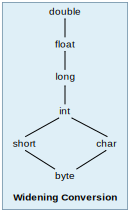
\includegraphics[width=.2\linewidth]{widening_type_conversion}}
	\end{example}
\end{frame}

\begin{frame}{Function \code{widenVar(a, t$_{out}$, t$_{in}$)}}
	\begin{definition}
		$\begin{array}{r@{}l}
			widenVar : \mathbb{A} \times \mathbb{T} \times \mathbb{T} \rightarrow & \mathbb{A} \\
			(a, t_{out}, t_{in}) \mapsto & \text{generates the code that widens the} \\
			& \text{value pointed by }a\text{ to the type }t_{out}\text{,} \\
			& \text{assuming that }a\text{ is of type }t_{in}\text{. This} \\
			& \text{conversion is done only if it is required.} \\
			& \text{Returns the address were the result} \\
			& \text{of the is available.} \\
		\end{array}$
	\end{definition}
\end{frame}

\begin{frame}{Example of Function \code{widenVar(a, t$_{out}$, t$_{in}$)}}
	Assume a language with only the two types \kw{int} and \kw{float}. \\
	\vspace{1em}
	\begin{myfunction}{widenVar}{a : $\mathbb{A}$, t$_{out}$ : $\mathbb{T}$, t$_{in}$ : $\mathbb{T}$}{$\mathbb{A}$}
		\Begin{
			\uIf{t$_{out}$ = t$_{in}$}{
				\Return a;
			}
			\uElseIf{t$_{in}$ = \kw{int} and t$_{out}$ = \kw{float}}{
				t \affect \kw{new} TemporaryVariable()\;
				quadruple(\str{'(float)'}, a, $\emptyset$, t)\;
				\Return t\;
			}
			\Else{
				\throw~\str{"Cannot widen the variable"}\;
			}
		}
	\end{myfunction}
\end{frame}

\begin{frame}{Function \code{narrowVar(a, t$_{out}$, t$_{in}$)}}
	\begin{definition}
		$\begin{array}{r@{}l}
			narrowVar : \mathbb{A} \times \mathbb{T} \times \mathbb{T} \rightarrow & \mathbb{A} \\
			(a, t_{out}, t_{in}) \mapsto & \text{generates the code that narrows the} \\
			& \text{value pointed by }a\text{ to the type }t_{out}\text{,} \\
			& \text{assuming that }a\text{ is of type }t_{in}\text{. This} \\
			& \text{conversion is done only if it is required.} \\
			& \text{Returns the address were the result} \\
			& \text{of the is available.} \\
		\end{array}$
	\end{definition}
\end{frame}

\begin{frame}{Example of Function \code{narrowVar(a, t$_{out}$, t$_{in}$)}}
	Assume a language with only the two types \kw{int} and \kw{float}. \\
	\vspace{1em}
	\begin{myfunction}{narrowVar}{a : $\mathbb{A}$, t$_{out}$ : $\mathbb{T}$, t$_{in}$ : $\mathbb{T}$}{$\mathbb{A}$}
		\Begin{
			\uIf{t$_{out}$ $\neq$ \kw{int} or t$_{in}$ $\neq$ \kw{float}}{
				\throw~\str{"Cannot narrow the variable"}\;
			}
			\uElseIf{t$_{out}$ = \kw{int} and t$_{in}$ = \kw{float}}{
				t \affect \kw{new} TemporaryVariable()\;
				quadruple(\str{'(float)'}, a, $\emptyset$, t)\;
				\Return t\;
			}
			\Else{
				\Return a\;
			}
		}
	\end{myfunction}
\end{frame}

\begin{frame}{Example of Type Conversions in SDD}
	The attribute "\code{type}" is added to store the type of an expression. \\
	The SDD is updated to check the types: \\
	\vspace{1em}
	\begin{sdd}
	\p{E ::= E \tok+ E}{	head.type = \alert{maxType}(E$_1$.type, E$_2$.type) \newl
				o1 = \alert{widenVar}(E$_1$.addr, E$_1$.type, head.type) \newl
				o2 = \alert{widenVar}(E$_2$.addr, E$_2$.type, head.type) \newl
				head.addr = \kw{new} TemporaryVariable() \newl
				quadruple( \str{'+'}, o1, o2, head.addr)}
	\p{E ::= \tok{id} \tok= E}{	head.addr = SymbolTable.getCurrent().get(\tok{id}.lexeme) \newl
					head.type = v.type \newl
					w = \alert{narrowVar}(E.addr, E.type, head.type) \newl
					\kw{if} (w $\neq$ E.addr) \newl
					\hspace{2em}\kw{warning}~\str{"May loose information"} \newl
					\kw{else} \newl
					\hspace{2em}w = \alert{widenVar}(E.addr, E.type, head.type) \newl
					quadruple(\str{'='}, w, $\emptyset$, head.addr)}
	\end{sdd}
\end{frame}

\subsubsection{Overloaded and polymorphic functions}

\tableofcontentslide[sections={3-6},sectionstyle={show/shaded},subsectionstyle={show/shaded/hide},subsubsectionstyle={show/shaded/hide/hide}]

\begin{frame}{Overloading of a Function}
	\begin{definition}
		Allows creating several functions with the same name, which differ from each other in the type of the input and the output of the function.
	\end{definition}
	\begin{itemize}
	\item Depending on the context, the overloading may be for a function, a procedure, a method, or an operator.
	\item \emph{The symbol table must contains all the signatures of the functions (in the context, which is using the symbol table).}
	\item A signature consists of:
		\begin{enumerate}
		\item the function name,
		\item the list of the types of the arguments of the function.
		\end{enumerate}
	\end{itemize}
\end{frame}

\begin{frame}{Polymorphic Function}
	\begin{definition}
			The term ``polymorphic'' refers to any code fragment that can be executed with arguments of different types.
	\end{definition}
	\vspace{2em}
	\begin{itemize}
	\item In this section, we consider the \emph{parametric polymorphism}, where the polymorphism is characterized by parameters or type variables.
	\end{itemize}
\end{frame}

\begin{frame}[fragile]{Example of Polymorphic Function}
	\begin{itemize}
	\item Consider the following definition in ML language:
		\begin{lstlisting}[language=ml]
		fun length(x) = if null(x) then 0 else length( tl(x) ) + 1;
		\end{lstlisting}
	\vfill
	\item Consider the following statement in ML language:
		\begin{lstlisting}[language=ml]
		length( ["sun", "mon", "tue"] ) + length( [10, 9, 8, 7] )
		\end{lstlisting}
	\vfill
	\item The same function \code{length()} is invoked on an array of strings and on an array of integers.
	\vfill
	\item The result of the ML statement is: \code{3 + 4 = 7}
	\end{itemize}
\end{frame}

\begin{frame}{Type of a Polymorphic Function}
	\begin{itemize}
	\item Using the symbol $\forall$ and the type constructor \kw{list}, the type of the function length can be written as:
		\begin{center}
			$\forall a.\kw{list}(a) \rightarrow \kw{int}$
		\end{center}
	\vfill
	\item The $\forall$ symbol is the universal quantifier, and the type variable to which it is applied is said to be bound by it.
	\item A type expression with a $\forall$ symbol in it will be referred as a ``polymorphic type.''
	\vfill
	\item Each time a polymorphic function is applied, its bound type variables (a\dots) can denote a different type.
	\end{itemize}
\end{frame}

\begin{frame}{Determining the Type of a Polymorphic Function}
	\alertbox{How to determine the types in the signature of a polymorphic function?}
	\vspace{1em}
	\alertbox*{We must infer the types by exploring the syntax tree of the function and applying the substitution and unification operations.}
	\begin{description}
	\item[Substitution] A mapping from type variables to type expressions. \inlineexample{\kw{list}(\kw{int}) is an instance of \kw{list}($\alpha$), since it is the result of substituting \kw{int} for $\alpha$ in \kw{list}($\alpha$).}
	\item[Unification] Determine whether type variables $s$ and $t$ are structurally equivalent by substituing the type variables in $s$ and $t$ by type expressions.
	\end{description}
\end{frame}

\begin{frame}[t,fragile]{Example of Type Inference on Polymorphic Function}
	\begin{columns}
		\begin{column}{.4\linewidth}
			\begin{small}
			\begin{lstlisting}[language=ml]
			fun length(x) =
			    if null(x) then 0
			    else length( tl(x) ) + 1;
			\end{lstlisting}
			\end{small}
		\end{column}
		\begin{column}{.6\linewidth}
			\begin{scriptsize}
			\begin{tabularx}{\linewidth}{|X|X|X|}
				\hline
				\tabularheading\chead{Expression}&\chead{Type}&\chead{Unification} \\
				\hline
				\only<1>{	& & \\ \hline}
				\only<2->{	length & $\beta \rightarrow \gamma$ & \\ \hline
						x & $\beta$ & \\ \hline}
				\only<3->{	\kw{if} & $\mathbb{B} \times \alpha \times \alpha \rightarrow \alpha$ & $\alpha = \gamma$\\ \hline}
				\only<4->{	null & $\kw{list}(\omega_n)\rightarrow\mathbb{B}$ & \\ \hline}
				\only<5->{	null(x) & $\mathbb{B}$ & $\kw{list}(\omega_n) = \beta$ \\ \hline}
				\only<6->{	0 & \kw{int} & $\alpha = \kw{int}$ \\ \hline}
				\only<7->{	\kw{+} & $\phi\times\phi\rightarrow\phi$ & $\phi = \alpha$ \\ \hline}
			\end{tabularx}
			\end{scriptsize}
		\end{column}
	\end{columns}
	\putat(-20,-200){\includeanimatedfigure[width=.4\paperwidth]{unification_example}}
	\only<8>{\putat(130,-125){\parbox{20em}{\mdseries\normalcolor\normalsize
		The type of the function "\code{length}" is: \\
		\code{length} : \kw{list}($\omega_n$) $\rightarrow$ \kw{int}
	}}}
\end{frame}

\section[Generation of statements]{Code generation of statements}

\tableofcontentslide[sections={3-},sectionstyle={show/shaded},subsectionstyle={show/show/hide},subsubsectionstyle={hide/hide/hide/hide}]

\subsection{Control flow}

\subsubsection{Introduction}

\tableofcontentslide[sections={3-},sectionstyle={show/shaded},subsectionstyle={show/shaded/hide},subsubsectionstyle={show/show/hide/hide}]

\begin{frame}{Control Flow}
	\begin{itemize}
	\item The translation of statements such as if-else-statements and while-statements is tied to the translation of boolean expressions.
	\item In programming languages, boolean expressions are often used to:
		\begin{enumerate}
		\item Alter the flow of control.
		\item Compute logical values.
		\end{enumerate}
	\item The intended use of boolean expressions is determined by its syntactic context.
	\item To support this distinction, we may:
		\begin{enumerate}
		\item Use two different nonterminals,
		\item Use inherited attributes,
		\item Use a set of flags during the parsing, or
		\item Build a syntax tree and invoke different procedures for the two different uses.
		\end{enumerate}
	\end{itemize}
\end{frame}

\begin{frame}[fragile]{Short-Circuit Code}
	\begin{itemize}
	\item In short-circuit code, the boolean operators translate into \emph{jumps}.
	\item The operators themselves do not appear in the code.
	\item Instead, the value of a boolean expression is represented by a position in the code sequence.
	\end{itemize}
	\begin{example}
		\begin{lstlisting}[linewidth=.6\linewidth,language=Java]
		if ( x < 100 || x > 200 && x != y ) x = 0;
		\end{lstlisting}
		\begin{tac}[.6\linewidth]
		\ifgoto{$x < 100$}{L1}
		\ifnotgoto{$x > 200$}{L2}
		\ifnotgoto{$x \neq y$}{L2}
		\a[L1]{$x$}{$0$}
		\tacdots[L2]
		\end{tac}
	\end{example}
\end{frame}

\subsubsection{Translate the control flow statements}

\tableofcontentslide[sections={3-},sectionstyle={show/shaded},subsectionstyle={show/shaded/hide},subsubsectionstyle={show/shaded/hide/hide}]

\begin{frame}{Statements for Control Flow}
	\begin{itemize}
	\item Consider the grammar:
		\raisebox{-.5\height}{
		\begin{footnotesize}
		\begin{bnf}[.5\linewidth]
		\p{S ::= \tok{if} \tok( B \tok) S}
		\p{  ::= \tok{if} \tok( B \tok) S \tok{else} S}
		\p{  ::= \tok{while} \tok( B \tok) S}
		\end{bnf}
		\end{footnotesize}}
	\vfill
	\item We introduce the attributes:
		\begin{itemize}
		\item \tactext{B.code} and \tactext{S.code}: synthesized attributes; three-address code of the nonterminals.
		\item \tactext{B.true}: inherited attribute; the label of the code associated to the then-statements.
		\item \tactext{B.false}: inherited attribute; the label of the code associated to the else-statements.
		\item \tactext{B.next}: inherited attribute; the label of the code just after the current if-then-else statements.
		\end{itemize}
	\end{itemize}
\end{frame}

\begin{frame}{Statement \kw{if}-\kw{then}}
	\begin{columns}
		\begin{column}{.4\linewidth}
			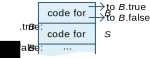
\includegraphics[width=\linewidth]{statement_if}
		\end{column}
		\begin{column}{.6\linewidth}
			\begin{footnotesize}
			\begin{sdd}
			\p{S ::= \tok{if} \tok(}{	B.true = newlabel() \newl
							B.false = head.next}
			\pcont{B \tok)}{		S.next = head.next \newl
							label(B.true)}
			\pcont{S}{}
			\end{sdd}
			\end{footnotesize}
		\end{column}
	\end{columns}
	\begin{itemize}
	\vfill
	\item The nontemirnal for the condition is no more $E$, but $B$.
	\item The function \tactext{newlabel()} creates a new label each time it is called.
	\item The function \tactext{label(L)} attaches label \tactext{L} to the next three-address instruction to be generated.
	\end{itemize}
\end{frame}

\begin{frame}{Statement \kw{if}-\kw{then}-\kw{else}}
	\begin{columns}
		\begin{column}{.4\linewidth}
			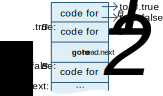
\includegraphics[width=\linewidth]{statement_if_else}
		\end{column}
		\begin{column}{.6\linewidth}
			\begin{footnotesize}
			\begin{sdd}
			\p{S ::= \tok{if} \tok(}{	B.true = newlabel() \newl
							B.false = newlabel()}
			\pcont{B \tok)}{		S$_1$.next = head.next \newl
							label(B.true)}
			\pcont{S \tok{else}}{		quadruple(\str{'goto'}, \newl
							\hspace{1em}head.next, \newl
							\hspace{1em}$\emptyset$, $\emptyset$) \newl
							S$_2$.next = head.next \newl
							label(B.false)}
			\pcont{S}{}
			\end{sdd}
			\end{footnotesize}
		\end{column}
	\end{columns}
\end{frame}

\begin{frame}{Statement \kw{while}}
	\begin{columns}
		\begin{column}{.4\linewidth}
			\includegraphics[width=\linewidth]{statement_while}
		\end{column}
		\begin{column}{.6\linewidth}
			\begin{footnotesize}
			\begin{sdd}
			\p{S ::= \tok{while} \tok(}{	begin = newlabel() \newl
							B.true = newlabel() \newl
							B.false = head.next}
			\pcont{B \tok)}{		S.next = begin \newl
							label(B.true)}
			\pcont{S}{			quadruple(\str{'goto'}, \newl
							\hspace{1em}begin, \newl
							\hspace{1em}$\emptyset$, $\emptyset$)}
			\end{sdd}
			\end{footnotesize}
		\end{column}
	\end{columns}
\end{frame}

\subsubsection{Boolean expressions for Control Flow}

\tableofcontentslide[sections={3-},sectionstyle={show/shaded},subsectionstyle={show/shaded/hide},subsubsectionstyle={show/shaded/hide/hide}]

\begin{frame}{Boolean Constants in the Control Flow}
	\begin{itemize}
	\item Boolean expressions dedicated to control flow need dedicated semantic rules.
	\item Remember that the boolean expressions used in control-flow statements must be translated into jumping three-address code.
	\end{itemize}
	\begin{sdd}
	\p{B ::= \tok{true}}{quadruple(\str{'goto'}, head.true, $\emptyset$, $\emptyset$)}
	\p{B ::= \tok{false}}{quadruple(\str{'goto'}, head.false, $\emptyset$, $\emptyset$)}
	\end{sdd}
\end{frame}

\begin{frame}{Boolean Operator NOT}
	\begin{columns}
		\begin{column}{.4\linewidth}
			\begin{center}
			\includegraphics[width=.5\linewidth]{statement_not}
			\end{center}
		\end{column}
		\begin{column}{.6\linewidth}
			\begin{footnotesize}
			\begin{sdd}
			\p{B ::= \tok{\string!} B}{	B.true = head.false \newl
							B.false = head.true}
			\end{sdd}
			\end{footnotesize}
		\end{column}
	\end{columns}
	\vfill
	\begin{itemize}
	\item No code is needed for an expression of the form \tactext{\tok{\string!}B}.
	\item Just interchange the \tactext{true} and \tactext{false} attributes of the head to set the \tactext{true} and \tactext{false} attributes of $B$.
	\end{itemize}
\end{frame}

\begin{frame}{Boolean Operator OR}
	\begin{columns}
		\begin{column}{.45\linewidth}
			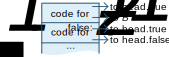
\includegraphics[width=\linewidth]{statement_or}
		\end{column}
		\begin{column}{.55\linewidth}
			\begin{footnotesize}
			\begin{sdd}
			\p{B ::=}{	B$_1$.true = head.true \newl
					B$_1$.false = newlabel()}
			\pcont{B}{	B$_2$.true = head.true \newl
					B$_2$.false = head.false}
			\pcont{\tok{\textbar\textbar} B}{}
			\end{sdd}
			\end{footnotesize}
		\end{column}
	\end{columns}
	\vfill
	\begin{itemize}
	\item If \bnftext{B$_1$} is true, the head is true.
	\item If \bnftext{B$_1$} is false, evaluate \bnftext{B$_2$}.
	\item So \bnftext{B$_1$.false} is the label of the first instruction of \bnftext{B$_2$}.
	\item The value of the head becomes the same as the value of \bnftext{B$_2$}.
	\end{itemize}
\end{frame}

\begin{frame}{Boolean Operator AND}
	\begin{columns}
		\begin{column}{.45\linewidth}
			\includegraphics[width=\linewidth]{statement_and}
		\end{column}
		\begin{column}{.55\linewidth}
			\begin{footnotesize}
			\begin{sdd}
			\p{B ::=}{	B$_1$.true = newlabel() \newl
					B$_1$.false = head.false}
			\pcont{B}{	B$_2$.true = head.true \newl
					B$_2$.false = head.false}
			\pcont{\tok{\&\&} B}{}
			\end{sdd}
			\end{footnotesize}
		\end{column}
	\end{columns}
	\vfill
	\begin{itemize}
	\item If \bnftext{B$_1$} is false, the head is false.
	\item If \bnftext{B$_1$} is true, evaluate \bnftext{B$_2$}.
	\item So \bnftext{B$_1$.true} is the label of the first instruction of \bnftext{B$_2$}.
	\item The value of the head becomes the same as the value of \bnftext{B$_2$}.
	\end{itemize}
\end{frame}

\begin{frame}{Operators of Comparison}
	\begin{columns}
		\begin{column}{.3\linewidth}
			\begin{center}
			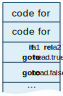
\includegraphics[width=.7\linewidth]{statement_rel}
			\end{center}
		\end{column}
		\begin{column}{.7\linewidth}
			\begin{footnotesize}
			\begin{sdd}
			\p{B ::= E \tok{rel} E}{	t = \kw{new} TemporaryVariable() \newl
							quadruple(\tok{rel}.operator, \newl
							\hspace{1em}E$_1$.addr, E$_2$.addr, t) \newl
							quadruple(\str{'if'}, t, \newl
							\hspace{1em}head.true, $\emptyset$) \newl
							quadruple(\str{'goto'}, head.false, \newl
							\hspace{1em}$\emptyset$, $\emptyset$)}
			\end{sdd}
			\end{footnotesize}
		\end{column}
	\end{columns}
	\vfill
	\begin{itemize}
	\item The form $a<b$ translates into: \\
		\tactext{t = ($a<b$)} \\
		\tactext{\kw{if} t \tok{then} \kw{goto} B.true} \\
		\tactext{\kw{goto} B.false} \\
	\end{itemize}
\end{frame}

\begin{frame}[fragile]{Example of Translation}
	\begin{lstlisting}[language=Java]
		if ( x < 100 || x > 200 && x != y ) x = 0;
	\end{lstlisting}
	\vfill
	\begin{tac}
	\a{\t1}{$x < 100$}
	\ifgoto{\t1}{L2}
	\goto{L3}
	\a[L3]{\t1}{$x > 200$}
	\ifgoto{$x > 200$}{L4}
	\goto{L1}
	\a[L4]{\t1}{$x \neq y$}
	\ifgoto{\t1}{L2}
	\goto{L1}
	\a[L2]{x}{0}
	\tacdots[L1]
	\end{tac}
\end{frame}

\subsubsection{Avoid redundant goto}

\tableofcontentslide[sections={3-},sectionstyle={show/shaded},subsectionstyle={show/shaded/hide},subsubsectionstyle={show/shaded/hide/hide}]

\begin{frame}{Redundant Goto Statements}
	\begin{small}
	\alertbox{The semantic rules described in the previous slides may generate more goto instructions than strictly necessary.}
	\begin{example}
		\begin{tac}
		\a[L3]{\t1}{$x>200$}
		\ifgoto{\t1}{L4}
		\goto{L1}
		\tacdots[L4]
		\tacdots[L1]
		\end{tac}
	\end{example}
	\begin{block}{Best Practice}
		\begin{tac}
		\a[L3]{\t1}{$x>200$}
		\ifnotgoto{\t1}{L1}
		\tacdots
		\tacdots[L1]
		\end{tac}
	\end{block}
	\end{small}
\end{frame}

\begin{frame}{Remove Redundant Gotos}
	\begin{itemize}
	\item Avoiding redundant gotos is done by introducing a constant for the value of the labels: \tactext{fall}.
	\item This constant means ``don't generate any jump.'', or ``fall in the next available instruction.''
	\vfill
	\item We can adapt the semantic rules of the boolean expressions. \bnftext{S \bnfbody \tok{if} \tok( B \tok) S}.
	\end{itemize}
	\begin{tabularx}{\linewidth}{@{}XcX@{}}
		\begin{scriptsize}
		\begin{sdd}
		\p{S ::= \tok{if} \tok(}{	B.true = newlabel() \newl
						B.false = head.next}
		\pcont{B \tok)}{		S.next = head.next \newl
						label(B.true)}
		\pcont{S}{}
		\end{sdd}
		\end{scriptsize}
		& \pgfuseimage{rightarrow}
		&
		\begin{scriptsize}
		\begin{sdd}
		\p{S ::= \tok{if} \tok(}{	B.true = \tok{fall} \newl
						B.false = head.next}
		\pcont{B \tok)}{		S.next = head.next}
		\pcont{S}{}
		\end{sdd}
		\end{scriptsize}
	\end{tabularx}
\end{frame}

\pgfdeclareimage[height=2em]{bottomarrow}{imgs/all/bottomarrow}

\begin{frame}{Remove Redundant Gotos of the OR Operator}
	\begin{center}
		\begin{footnotesize}
		\begin{sdd}[.7\linewidth]
		\p{B ::=}{	B$_1$.true = head.true \newl
				B$_1$.false = newlabel()}
		\pcont{B}{	B$_2$.true = head.true \newl
				B$_2$.false = head.false}
		\pcont{\tok{\textbar\textbar} B}{}
		\end{sdd}
		\end{footnotesize} \\[1em]
		\pgfuseimage{bottomarrow} \\[1em]
		\begin{footnotesize}
		\begin{sdd}[.7\linewidth]
		\p{B ::=}{	\kw{if} head.true = \kw{fall} \newl
				\hspace{1em}B$_1$.true = newlabel() \newl
				\kw{else} \newl
				\hspace{1em}B$_1$.true = head.true \newl
				B$_1$.false = \kw{fall}}
		\pcont{B}{	B$_2$.true = head.true \newl
				B$_2$.false = head.false}
		\pcont{\tok{\textbar\textbar} B}{
				\kw{if} head.true = \kw{fall} \newl
				\hspace{1em}label(B$_1$.true)}
		\end{sdd}
		\end{footnotesize}
	\end{center}
\end{frame}

\subsection{Backpatching}

\subsubsection{Introduction}

\tableofcontentslide[sections={3-},sectionstyle={show/shaded},subsectionstyle={show/shaded/hide},subsubsectionstyle={show/show/hide/hide}]

\begin{frame}[allowframebreaks]{Problem with Jumps}
	\alertbox{A key problem is the matching of a jump instruction with the target address of the jump.}
	\vspace{1em}
	\begin{example}
		\begin{itemize}
		\item Consider the statement \bnftext{\tok{if} \tok( B \tok) S}.
		\item In a \emph{one-pass translation}, $B$ must be translated before $S$ is examined.
		\item \emph{What is the address of the label that permits to go over the code for $S$?}
		\end{itemize}
	\end{example}
	%
	\framebreak
	%
	\begin{block}{Solution 1}
		\begin{itemize}
		\item In the previous slides, we solve this problem by using inherited attributes "\texttt{next}".
		\item \alert{But a separate pass is then needed to bind labels to addresses.}
		\end{itemize}
	\end{block}
	\vspace{1em}
	\begin{block}{Solution 2}
		\begin{itemize}
		\item \emph{Backpatching} can be used to generate code for boolean expressions and flow-of-control statements in one pass.
		\item This approach is detailled in the following slides.
		\end{itemize}
	\end{block}
\end{frame}

\begin{frame}{General Principle of Backpatching}
	\begin{itemize}
	\item When the jump target is after the current instruction, the address of the current instruction is added into a list.
	\vspace{2em}
	\item When the address of the target instruction is known, the instructions in the list are updated.
	\end{itemize}
\end{frame}

\begin{frame}{New attributes for the Backpatching}
	\begin{itemize}
	\item Introduction of synthesized attributes: \emph{bptruelist} and \emph{bpfalselist} of the nonterminal $B$ are used to manage labels in jumping code for \emph{boolean expressions}.
	\vfill
		\begin{description}
		\item[B.bptruelist] list of jump or conditional jump instructions into which we must insert the label to which control goes if $B$ is true.
	\vfill
		\item[B.bpfalselist] list of instructions that eventually get the label to which control goes when $B$ is false.
		\end{description}
	\vfill
	\item Similarly, the other productions, such as $S$, must be updated in a simular way with synthesized attributes.
	\end{itemize}
\end{frame}

\begin{frame}{Tools for the Backpatching}
	\begin{description}
	\item[makebplist(adr)] creates a new list containing only $adr$, an index into the array of instructions.
	\vfill
	\item[mergebplists(lst1,lst2)] concatenates the lists pointed by $lst1$ and $lst2$, and returns a pointer to the result.
	\vfill
	\item[backpatch(lst,adr)] inserts $adr$ as the target label for each of the instructions on the list pointed to by $lst$.
	\vfill
	\item[instadr()] replies the address of the instruction that will be generated by the \Emph{next} call to \tactext{quadruple()}.
	\vfill
	\item[Unknown address] The keyword \kw{?} represents an unkwown address.
	\end{description}
\end{frame}

\begin{frame}{Backpatching of the Boolean Control-Flow Rules}
	\begin{sdd}
	\p{B ::= \tok{true}}{	\emph{head.bptruelist = makebplist(instadr())} \newl
				quadruple(\str{'goto'}, \emph{\kw{?}}, $\emptyset$, $\emptyset$)}
	\hline
	\p{B ::= \tok{false}}{	\emph{head.bpfalselist = makebplist(instadr())} \newl
				quadruple(\str{'goto'}, \emph{\kw{?}}, $\emptyset$, $\emptyset$)}
	\hline
	\p{B ::= E \tok{rel} E}{	t = \kw{new} TemporaryVariable() \newl
					quadruple(\tok{rel}.operator, E$_1$.addr, E$_2$.addr, t) \newl
					\emph{head.bptruelist = makebplist(instadr())} \newl
					quadruple(\str{'if'}, t, \emph{\tok{?}}, $\emptyset$) \newl
					\emph{head.bpfalselist = makebplist(instadr())} \newl
					quadruple(\str{'goto'}, \emph{\tok{?}}, $\emptyset$, $\emptyset$)}
	\hline
	\p{B ::= B \tok{\textbar\textbar}}{	\emph{backpatch(B$_1$.bpfalselist, instadr())}}
	\pcont{B}{				\emph{head.bptruelist = mergbplists(} \newl
						\hspace{1em}\emph{B$_1$.bptruelist, B$_2$.bptruelist)} \newl
						\emph{head.bpfalselist = B$_2$.bpfalselist}}
	\end{sdd}
\end{frame}

\begin{frame}{Backpatching of the Control-Flow Statements}
	\begin{small}
	\begin{sdd}
	\p{S ::= \tok{if} \tok( B \tok)}{	backpatch(B.bptruelist, instadr())}
	\pcont{S}{				head.\emph{bpnextlist} = mergebplists(B.bpfalselist, S.\emph{bpnextlist})}
	\hline
	\p{S ::= \tok{if} \tok( B \tok)}{	backpatch(B.bptruelist, instadr())}
	\pcont{S \tok{else}}{			backpatch(B.bpfalselist, instadr())}
	\pcont{S}{				head.\emph{bpnextlist} = mergebplists(S$_1$.\emph{bpnextlist}, S$_2$.\emph{bpnextlist})}
	\hline
	\p{S ::= \tok{while}}{		a = instadr()}
	\pcont{\tok( B \tok)}{		backpatch(B.bptruelist, instadr())}
	\pcont{S}{			backpatch(S.\emph{bpnextlist}, a) \newl
					quadruple(\str{'goto'}, a, $\emptyset$, $\emptyset$) \newl
					head.\emph{bpnextlist} = B.bpfalselist}
	\end{sdd}
	\vfill
	The attribute \tactext{bpnextlist} is the list of the addresses of the instructions that are refering the ``next instruction.''
	\end{small}
\end{frame}

\begin{frame}{Algorithm of \code{backpatch()}}
	\begin{scriptsize}
	\begin{myprocedure}{backpatch}{list, address}
	\Input{$\mathbb{Q}$ is the global list of the generated quadruples.}
	\Begin{
		\ForEach{$a \in list$}{
			q \affect $\mathbb{Q}[a]$\;
			\uIf{q.op = \str{'goto'}}{
				\lIf{q.arg$_1$ $\neq$ \kw{?}}{\throw~\str{"Cannot backpatch"}}\;
				q.arg$_1$ \affect address\;
			}
			\uElseIf{q.op = \str{'if'}}{
				\lIf{q.arg$_2$ $\neq$ \kw{?}}{\throw~\str{"Cannot backpatch"}}\;
				q.arg$_2$ \affect address\;
			}
			\uElseIf{q.op = \str{'ifFalse'}}{
				\lIf{q.arg$_2$ $\neq$ \kw{?}}{\throw~\str{"Cannot backpatch"}}\;
				q.arg$_2$ \affect address\;
			}
			\Else{
				\throw~\str{"Instruction to backpatch not found"}\;
			}
		}
	}
	\end{myprocedure}
	\end{scriptsize}
\end{frame}

\section{Conclusion}

\tableofcontentslide[sectionstyle={show/shaded},subsectionstyle={hide/hide/hide},subsubsectionstyle={hide/hide/hide/hide}]

\begin{frame}[t,allowframebreaks]{Key Concepts in the Chapter}
	\begin{description}
	\item[Inherited and synthesized attributes] Syntax-directed definitions may use two kinds of attributes. A synthesized attribute at a parse-tree node is computed from attributes at its children. An inherited attribute at a node is computed from attributes at its parent and/or siblings.
	\item[Dependency graphs] Given a parse tree and an SDD, we draw edges among the attribute instances associated with each parse-tree node to denote that the value of the attribute at the head of the edge is computed in terms of the value of the attribute at the tail of the edge.
	\item[S-Attributed definitions] In a S-attributed SDD, all attributes are synthesized.
	\item[L-Attributed definitions] In a L-attributed SDD, attributes may be inherited or synthesized. However, inherited attributes at a parse-tree node may depend only on inherited attributes of its parent and on (any) attributes of siblings to its left.
Syntax trees: Each node in a syntax tree represents a construct; the children of the node represent the meaningful components of the construct.
	\item[Intermediate representation] An intermediate representation is typically some combination of a graphical notation and three-address code. As in syntax, a node in a graphical notation represents a construct; the children of a node represent its subconstructs. Three address code takes its name from instructions of the form \tactext{x = y \kw{op} z}, with at most one operator per instruction. There are additional instructions for control flow.
	\item[Translate expressions] Expressions with built-up operations can be unwound into a sequence of individual operations by attaching actions to each production of the form \bnftext{E \bnfbody E$_1$ \tok{op} E$_2$}. The action either creates a node for \bnftext{E} with the nodes for \bnftext{E$_1$} and \bnftext{E$_2$} as children, or it generates a three-address instruction that applies op to the addresses for \bnftext{E$_1$} and \bnftext{E$_2$} and puts the result into a new temporary name, which becomes the address of \bnftext{E}.
	\item[Check types] The type of an expression \tactext{E$_1$ \kw{op} E$_1$} is determined by the operator \kw{op} and the types of \tactext{E$_1$} and \tactext{E$_2$}. A coercion is an implicit type conversion. Intermediate code contains explicit type conversions to ensure an exact match between operand types and the types expected by an operator.
	\item[Generate jumping code for boolean expression] In short-circuit or jumping code, the value of a boolean expression is implicit in the position reached in the code. Jumping code is useful because a boolean expression $B$ is typically used to \tactext{t=true} or \tactext{t=false}, as appropriate, where \tactext{t} is a temporary name. Using labels for jumps, a boolean expression can be translated by inheriting labels corresponding to its true and false exits attributes. The constants \kw{true} and \kw{false} translate into a jump to the true and false attributes, respectively.
	\item[Implement statements using control flow] Statements can be translated by inheriting a label next, where next marks the first instruction after the code for this statement. The conditional \bnftext{S \bnfbody \tok{if} \tok( B \tok) S} can be translated by attaching a new label marking the beginning of the code for \bnftext{S} and passing the new label and \tactext{S.next} for the true and false attributes, respectively, of $B$.
	\item[Alternatively, use backpatching] Backpatching is a technique for generating code for boolean expressions and statements in one pass. The idea is to maintain lists of incomplete jumps, where all the jump instructions on a list have the same target. When the target becomes known, all the instructions on its list are completed by filling in the target.
	\item[Implement records] Field names in a record or class can be treated as a sequence of declarations. A record type encodes the types and relative addresses of the fields. A symbol table object can be used for this purpose.
	\end{description}
\end{frame}

\begin{frame}[t,allowframebreaks]{\bibname\ of the Chapter}%
	\tiny%
	\putbib[bibliographies/chapter4]%
\end{frame}%

\end{bibunit}

% Reset the style of the navigation box
\setbeamertemplate{headline text style}{}

